\documentclass[a4paper, oneside, english]{sapthesis} % or twoside
% add noexaminfo to the options to hide information about graduation seession

% Sapthesis explicitely loads the packages:
% xkeyval, etoolbox, geometry, ifxetex, xltxtra, fontenc, textcomp,
% lmodern, caption, graphicx, color, booktabs, amsmath, fancyhdr.
% DO NOT include them again.

% original editor style: textmate

\usepackage[hidelinks]{hyperref}
\usepackage{amssymb}
\usepackage{comment}
\usepackage{booktabs}
\usepackage{multirow}
\usepackage{caption}
\usepackage{xcolor}         % custom colors
\usepackage{subcaption}
\usepackage{wrapfig}        % to wrap figures in text
\usepackage{float}          % to support previous one
\usepackage{enumerate}      % to enable custom bullets
\usepackage{minted}         % code blocks
%\usepackage{arydshln} % to use dashed lines in tables

\definecolor{customgreen}{HTML}{00B050} % 92DD5F
\definecolor{commentcol}{rgb}{0.3, 0.6, 0.6}

\renewcommand{\bibname}{References} % change Bibliography title to References

\title{Benchmarking CLIP Models for Remote Sensing \\Applications}
%\subtitle{...}
\author{Cristiana Di Tullio}
\IDnumber{1803880}
\course{Master's Degree in Data Science}
\courseorganizer{Facoltà di Ingegneria dell'Informazione, Informatica e Statistica}
\AcademicYear{2024/2025}
\advisor{Simone Scardapane}
\coadvisor{Marco Montagna}
\examdate{18th July 2025}
\examiner[]{Pierpaolo Brutti} % use [] to specify role (default:chairman)
\examiner{Mattia Crespi}
\examiner{D'Ecclesia Rita Laura}
\examiner{Francesco Leotta}
\examiner{Pompeo Polito}
\examiner{Walter Quattrociocchi}
\examiner{Simone Scardapane}
\thesistype{Master thesis}
\copyyear{2025}
\authoremail{ditullio.1803880@studenti.uniroma1.it}
\date{\today}

\begin{document}

\frontmatter
\maketitle
\dedication{(add a dedication)}

%\abstract{(add an abstract)}
% Use the following environment instead
\begin{abstract}
    (add an abstract)
\end{abstract}

\tableofcontents

\mainmatter

\chapter{Introduction} % -------------------------------------
% Keep in mind: 
% - the topic is Machine Learning (SSL specifically)
% - clarify research questions and contributions, to take up again in the conclusion

In broad terms, Remote Sensing is the process of acquiring information from a distance using appropriate satellite or aerial instrumentation. As a field of study, it has gained increasing attention over the past few years, demonstrating to play a fundamental role in agriculture, meteorology, environmental science, not to mention large-scale and impactful social challenges such as climate change, urbanization and disaster management. In contrast to conventional computer vision domains, Remote Sensing features a unique kind of data, inherently multimodal: in fact, satellite imagery is captured through different types sensors like optical (multispectral and hyperspectral), Lidar and SAR, which capture complex geophysical elements and are collected at high spatial and temporal resolutions. These images span different sets of multiple spectral bands and are highly rich in metadata related to georeferencing, topographic and geodetic measurements, which serve as the primary source of information for many and diverse types of analyses. Moreover, Remote Sensing increasingly faces the big data problem as terabytes of satellite images are captured every day and need to be organized and processed in efficient and scalable ways. The time variable is becoming increasingly crucial. In this context, Deep Learning can make a massive contribution providing flexible and domain-adaptive models to tackle specialized tasks \cite{zhu2017deep}.

In recent times, the Deep Learning subfield of Computer Vision (CV) has witnessed unprecedented advancements. The most famous and fundamental Computer Vision models are undoubtedly Convolutional Neural Networks (CNNs), built in the context of supervised learning, that can be easily trained on vast labeled datasets and achieve state-of-the-art performance on a wide range of visual tasks from object detection to scene understanding and semantic segmentation. However, despite being highly effective for specific tasks, these models entail two major limitations: first, all supervised learning approaches require labeled datasets, and it can be surprisingly hard to assemble a comprehensive Remote Sensing dataset of good quality due to the remarkable need of human and computational effort to preprocess and carefully annotate satellite images, which is a highly costly and often impractical process; secondly, the performance of supervised models is tied to the nature and scope of their training data, i.e. they are typically trained to predict from a fixed set of categories and can't handle new classes or distributional shifts: every minor modification in the desired behaviour would imply modifying the training dataset, and this is unfeasible for the above reasons.

In this context, the advent of Vision-Language Models (VLMs) has revolutionized Computer Vision \cite{marimo2025beyond} introducing powerful zero-shot generalization capabilities and great cross-modal performances. VLMs are powerful deep learning multimodal models that bridge the gap between text and visual data such as images or videos, allowing to address complex tasks such as image generation from text prompts or image captioning from visual inputs. To be able to fulfill these and other functions, VLMs typically include two essential components: a vision encoder and a language encoder. Then, different training strategies can be adopted to learn how to align information from the two different data modalities, some of the most popular being Contrastive Learning \cite{radford2021learning} \cite{chen2020simple} \cite{he2020momentum} \cite{jia2021scaling}, Masking \cite{singh2022flava}, Generative Model Pretraining \cite{ramesh2022hierarchical} \cite{rombach2022high} \cite{saharia2022photorealistic} \cite{alayrac2022flamingo}. In particular, this thesis work focuses on \emph{CLIP (Contrastive Language–Image Pretraining)} \cite{radford2021learning}, a self-supervised VLM introduced by OpenAI in 2021. CLIP and derived models differ from traditional CNN pipelines in belonging to the category of Self-Supervised Learning algotirhms, specifically Contrastive Learning, and in being multimodal models able to align visual and textual representations in a shared embedding space. Moreover, the original model exhibits stunning zero-shot abilities which are the reason why it is still one of the most widely used and appreciated models in cross-modal applications, despite some may consider it slightly "old" now (given the current rate of release of new machine learning models). While CLIP may not achieve top-tier accuracy on every benchmark when compared to task-specific models like CNNs, its generalization capabilities and support for natural language labels make it an unrivaled versatile tool for its versatility.

This thesis explores the prospects of CLIP-like models in the Remote Sensing domain, where these properties are particularly valuable given the non-trivial nature of the data and the applications. The baseline performance of CLIP and its domain-specialized variants \cite{liu2024remoteclip} \cite{zhang2024rs5m} \cite{wang2024skyscript} is assessed on a suite of remote sensing benchmark datasets. Nevertheless, a fundamental challenge remains: CLIP and its derivatives are intrinsically limited to RGB imagery, while most satellite data contain a higher amount of information spanning across multiple bands of the electromagnetic spectrum (e.g., near-infrared, shortwave infrared). These additional bands can capture features invisible to the human eye that are essential for many remote sensing tasks, holding a great unexploited potential. However, it's not trivial to leverage this rich information within the CLIP framework as the model is neither designed nor trained to process multispectral inputs (MSI). A straightforward solution would be to re-train a CLIP-like model entirely on multispectral data \cite{marimo2025beyond} or to finetune it, but both these ideas come together with high costs of time and resources. Instead, this work proposes a comparatively lightweight and scalable solution to integrate multispectral information into CLIP-like models without the computational burden of retraining the entire architecture. Specifically, we introduce a modular MSI embedder that projects multispectral inputs into a 3-channel representation compatible with CLIP's original RGB-only image encoder. By training only this embedder while keeping the rest of CLIP frozen, we aim to enhance model performance with minimal computational effort, exploiting the full spectral data abundance of remote sensing images.

The research questions at the core of this work are:

\begin{enumerate}
    \item How well do existing CLIP-like models perform in zero-shot classification on standard RGB remote sensing datasets?
    \item Is it possible to improve CLIP’s classification performance in remote sensing by integrating multispectral data through a lightweight embedder?
    \item Can this approach generalize across datasets, i.e. and lends itself to transfer learning scenarios?
\end{enumerate}

To answer such questions, a series of experiments was conducted along three main directions: benchmarking zero-shot performance of various CLIP-based models on RGB imagery, developing and evaluating two variants of the MSI embedder (namely MSI1 and MSI2), exploring different image normalization techniques and transfer learning setups to implement a model with good generalization capabilities. We found that integrating multispectral information via the proposed approach consistently matches or improves classification accuracy over RGB-only baselines after finetuning and also the transfer learning idea succeeded in certain configurations - highlighting the potential of this lightweight, plug-and-play strategy and paving the way for further enhancement of VLMs integrating MSI information in the remote sensing domain.

\chapter{Related Works} % --------------------------------------

\section{CLIP in Remote Sensing}

Vision-Language Models and specifically CLIP-style contrastive pretraining methods have mostly started to gain popularity in Earth Observation (EO) only in the last couple of years: nevertheless, many great contributions have been made to this specific area of study in the meantime with promising results in terms of both datasets and models. Although, almost all the work done remained confined to RGB imagery and was only optimized for this kind of input data, and we feel that it is not enough: it is worth to highlight that even the best performing CLIP-like model in the field of Remote Sensing never surpasses accuracy values of just $60-70\%$ on satellite images benchmarks. In the writer's opinion, there is much room for improvement - and exploiting the additional remote sensing information will be key. A crucial issue lies in that Earth Observation (EO) data often lack suitable natural language captions or description and tend to include only categorical labels or metadata. While some approaches have been tried out to generate captions automatically, they mostly include annotations based on metadata and/or curated by humans, as is the case with the famous RSITMD \cite{yuan2022exploring}, RSICD \cite{lu2017exploring} and UCM \cite{yang2010bag}; being too limited in size to support training ($< 10,000$ samples), they are mainly used for evaluation purposes. Larger efforts feature BigEarthNet \cite{sumbul2019bigearthnet}, a broad archive first proposed in 2019 comprising approximately $590,000$ Sentinel‑2 patches with multi-label land-cover annotations covering 43 classes; this datasets was later extended to include Sentinel‑1 data in the BigEarthNet‑MM version from 2021 \cite{sumbul2021bignearthnetmm} for a total of $590,326$ patches, enabling multi-modal analysis across SAR and optical bands for the same geographic tiles; then, it was further refined into reBEN \cite{clasen2024reben} later this year, containing $549,488$ pairs of Sentinel-1 and Sentinel-2 high quality image patches of size 1200 m x 1200 m. Other prominent works include RSCLIP \cite{li2023rs} which introduced a pseudo-labeling technique to finetune the CLIP model on RS images; the RS5M dataset \cite{zhang2024rs5m} which managed to reach a dimension of $5$ millions of image-text samples employing BLIP-2 \cite{li2023blip} to generate captions; the SkyScript dataset \cite{wang2024skyscript} leveraged geocoordinates to connect images to the rich semantics provided by OpenStreetMap, accounting for $2.6$ million image-text pairs covering 29K distinct conceptual tags; ChatEarthNet \cite{yuan2024chatearthnet} was the first dataset including diverse imagery and employing models of the ChatGPT family to generate image descriptions, for a total of $163488$ images captioned with ChatGPT-3.5 and $10000$ additional pairs captioned by ChatGPT-4V. Even so, all these approaches remain fundamentally RGB-only, missing out on the rich spectral information captured by multispectral or hyperspectral sensors. However, it is worth noticing that the value of MSI information is starting to gather more and more interest in recent times: the Major TOM (Terrestrial Observation Metaset) dataset \cite{francis2024major} was part of an initiative by ESA $\Phi$-lab to standardize and unify large-scale EO datasets based on a global 10km $\times$ 10km grid including millions of satellite image patches, divided in sets differentiated by sensor data spannig across both Sentinel-1 (radar) and Sentinel-2 (optical) for highly composite spectral images; finally, as of just a few months ago, TerraMesh \cite{blumenstiel2025terramesh} marked another significant leap forward introducing a massive globally distributed, multimodal dataset with over $9$ million co-registered samples, including optical, SAR and elevation data, NDVI indexes and land-cover maps - all preprocessed in an analysis and pre-training ready form.

These datasets, although offering rich, multispectral grounding, are not accompanied by suitable text captions to leverage the full potential of VLMs relying on contrastive learning and the current CLIP-based landscape for remote sensing remains limited to RGB-only inputs.


\section{RGB approaches}

To adapt CLIP to the earth observation domain without redesigning its core, several methods have fine-tuned CLIP backbones on remote sensing-specific datasets of RGB images captioned with various techniques, ranging from manually to semi-automatic and fully automatic annotation approaches. The most significant contributions include:

\begin{itemize}
    \item \emph{RemoteCLIP (2023)} \cite{liu2024remoteclip}: the first large-scale application of CLIP to remote sensing, is a \emph{foundation model} which builds an image–caption corpus from bounding-box and segmentation annotations using Box‑to‑Caption and Mask‑to‑Box conversions, augmented with UAV imagery—12× larger than prior datasets. This enabled zero-shot classification, retrieval, k‑NN, few-shot tasks, and novel object counting, achieving up to $6.4\%$ improvement in accuracy and $\sim 9\%$ recall gains in retrieval;
    \item \emph{SkyCLIP (late 2023)} \cite{wang2024skyscript}: finetuned on the SkyScript dataset and released at the publication of the paper as part of the experiments, it consistently outperformed RemoteCLIP in scene classification and fine-grained classification tasks;
    \item \emph{GeoRSCLIP (early 2024)} \cite{zhang2024rs5m}: pre-trained on RS5M, it achieved state-of-the-art performances surpassing RemoteCLIP in all the relevant benchmarks providing robust downstream performance;
    \item \emph{RS-M-CLIP (2024)} \cite{silva2024multilingual}: a multilingual variant of CLIP trained on translated captions, achieving state‑of‑the‑art cross-modal multilingual retrieval and zero-shot classification performance. It supports nine other languages in addition to English (German, French, Spanish, Chinese, Portuguese, Italian, Russian, Korean, and Dutch);
    \item \emph{PIR-CLIP (2024)} \cite{pan2024pir}: this model enhanced retrieval via “prior instruction” learning, targeting improved text representation and semantic clarity. Again surpassed the state-of-the-art performance in cross-modal image-to-text and text-to-image retrieval tasks, improving on the precedent models as shown in Figure \ref{fig:pirclip};
    \item \emph{SEN-CLIP (late 2024)} \cite{jain2025senclip}: this model focused on Sentinel‑2 imagery and adopted specialized pooling strategies, obtaining $10\%+$ accuracy increases over prior CLIP variants up to GeoRSCLIP for classification. However, a comprehensive comparison with PIR-CLIP and other models on classic cross-modal retrieval tasks is missing.
\end{itemize}

\begin{figure}[h]
    \centering
    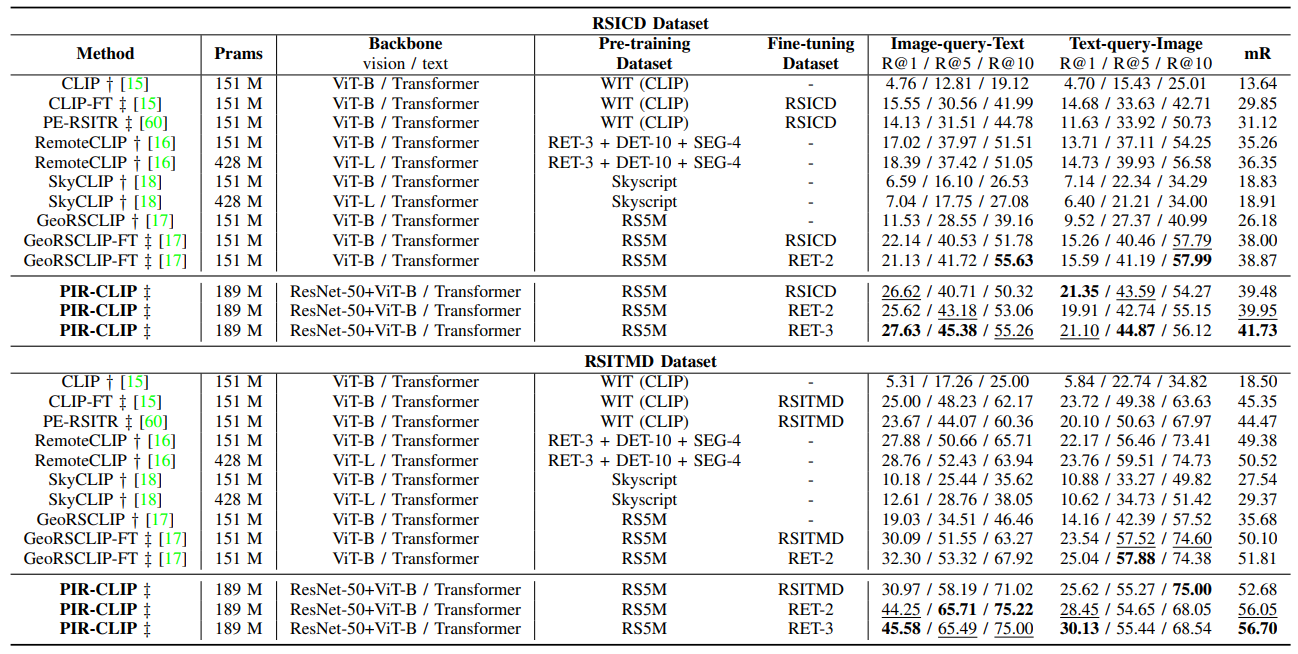
\includegraphics[width=\textwidth]{img/PIRCLIP_summary_results.png}
    \caption{Comparison of model performance on standard image-to-text and text-to-image retrieval datasets RSICD \cite{lu2017exploring} and RSITMD \cite{yuan2022exploring}. Despite not being strictly correlated to classification performances, this task is more common in evaluation of remote sensing CLIP-like models and the most documented one for performance cross-checking. As of the original paper \cite{pan2024pir}, $\dagger$ represents zero-shot CLIP and $\ddagger$ fine-tuned CLIP.}
    \label{fig:pirclip}
\end{figure}


So, a plurality of models has already been proposed. They all share a common methodological pipeline: collect RS image–caption pairs with more or less sophisticated techniques, fine-tune CLIP vision and text encoders via contrastive loss, and achieve more and more significant gains over vanilla CLIP. However, they all remain RGB-bound, ignoring multispectral information in datasets with up to $13$ spectral bands like Sentinel‑2. Moreover, the fine-tuning process is computationally demanding and typically requires large-scale domain-specific data, which is why many of these models have been presented as a result of studies about construction of remote sensing \emph{datasets}. Efficiency on standard hardware is also limited by the increasing model sizes.


\section{MSI approaches}

According to the literature, only one work so far has dared to adventure into the domain of multispectral bands incorporating them into a CLIP model training process and underscoring the value of MSI data. A pioneering research conducted at IBM later this year: 

\begin{itemize}
    \item \emph{Llama3‑MS‑CLIP3 (2025)} \cite{marimo2025beyond}: this is a multispectral CLIP built via continued pretraining on a novel dataset created for the occasion, containing $\sim 1$ million of Sentinel 2‑based images captioned automatically using Llama3-LLaVA-Next \cite{li2024llava}, Overture Maps data and SSL4EO-S12 \cite{wang2023ssl4eo} metadata. This variant achieved superior zero-shot classification and textual retrieval performance, outperforming RGB-based counterparts across multiple benchmarks as shown in Figure \ref{fig:msclip}.
\end{itemize}

\begin{figure}[h]
    \centering
    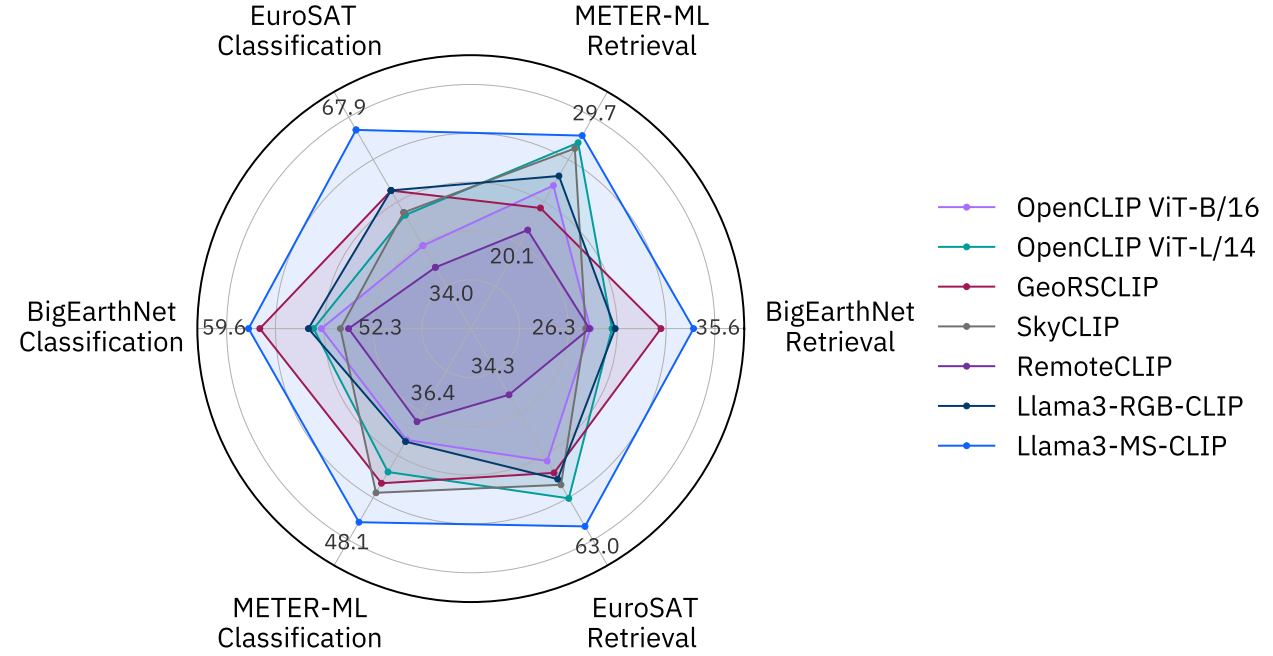
\includegraphics[width=0.8\textwidth]{img/MS-CLIP.png}
    \caption{Zero-shot classification and text-to-image retrieval results, measured respectively in accuracy and mAP percentages. The multispectral CLIP outperforms other RGB-based models on most of the benchmarks tested \cite{marimo2025beyond}.}
    \label{fig:msclip}
\end{figure}

This approach clearly demonstrates the effectiveness of multispectral input. Although, it comes at a high computational cost: large infrastructure, significant GPU hours for training and complex caption-generation pipelines. At the time this thesis is being compiled, assets remain unreleased, which limits reproducibility. Therefore, and even more so, we respond to the need of a more lightweight and usable solution. In the following chapters, we explore a different strategy to leverage multispectral richness while retaining the zero-shot and fine-tunable capabilities of CLIP-like models.


%\chapter{Vision Language Models}  % ---------------------------

%Vision Language Models explained on HF: https://huggingface.co/blog/vlms

%\section{Residual Networks backbone (ResNet)}
%\subsection{Convolutional Neural Networks}
%\subsection{The ResNet architecture}

%\section{Vision Transformer backbone (ViT)}
%\subsection{The Transformers architecture}
%\subsection{The Multi-Head Self-Attention mechanism}

\chapter{The CLIP model} % ------------------------------------

The OpenAI's \textbf{CLIP (Contrastive Language-Image Pre-Training)} model \cite{radford2021learning} was presented in 2021 and represents a pivotal leap in Vision-Language modeling, designed to learn a unified representation of images and texts. By jointly training on a large-scale diverse dataset of images and their corresponding textual descriptions, CLIP encodes both modalities into a shared embedding space, learning a combined representation that is ideal for many cross-modal purposes without requiring a specific fine-tuning. As a result, the model proves incredibly flexible and effective across image classification, image-to-text or text-to-image retrieval, image segmentation, object detection tasks and more.

The core working principle behind CLIP is \emph{Contrastive Learning} (CL), a methodology that falls under the umbrella of Self Supervised Learning (SSL). In conceptual terms, the model is trained to maximize the similarity between matching image-text pairs and minimize the similarity between mismatched pairs. This approach enables meaningful cross-modal alignment and allows the model to generalize to unseen data and tasks involving an open vocabulary, making it highly versatile for real-world applications. In Figure \ref{fig:clip} the overall structure of CLIP is displayed: this model comprises two encoders for the two different input modalities, and pre-trains them together to align the similar input pairs leveraging the InfoNCE contrastive loss function. Once the inputs are encoded in the shared embedding space, the dot product calculates the similarity between the embeddings.

CLIP yields a number of notable benefits:

\begin{itemize}
    \item It can deal with any piece of text from single words to full sentences, going beyond specific class labels. In fact, it can be prompted in natural language;
    \item It has a strong understanding of general textual and visual concepts, thanks to the huge amount of data it was pre-trained on;
    \item The text descriptors it was pre-trained on often describe various elements within an image, both in the foreground and in the background, enabling the model to recognize not only a picture's subject but also the context.
\end{itemize}

These are the primary factors that have led to CLIP's great success in Vision-Language modeling and its key role in many multimodal applications, including guide image generation processes in other models like the DALL-E family \cite{ramesh2022hierarchical} and Stable Diffusion \cite{rombach2022high}.


\section{The CLIP architecture}

The CLIP model is built around a symmetric dual-encoder architecture, visible in Figure \ref{fig:clip}. This scheme is designed to independently process and embed visual and textual data into a common feature space. The core principle behind this design is modality separation followed by alignment: each input modality, image or text, is first encoded via its own specialized backbone, and then mapped into a shared latent space where similarity can be computed directly. It is worth remarking that CLIP is \textit{not} a generative model: it is necessary to feed it \textit{both} visual and language inputs.

\begin{figure}[h]
    \centering
    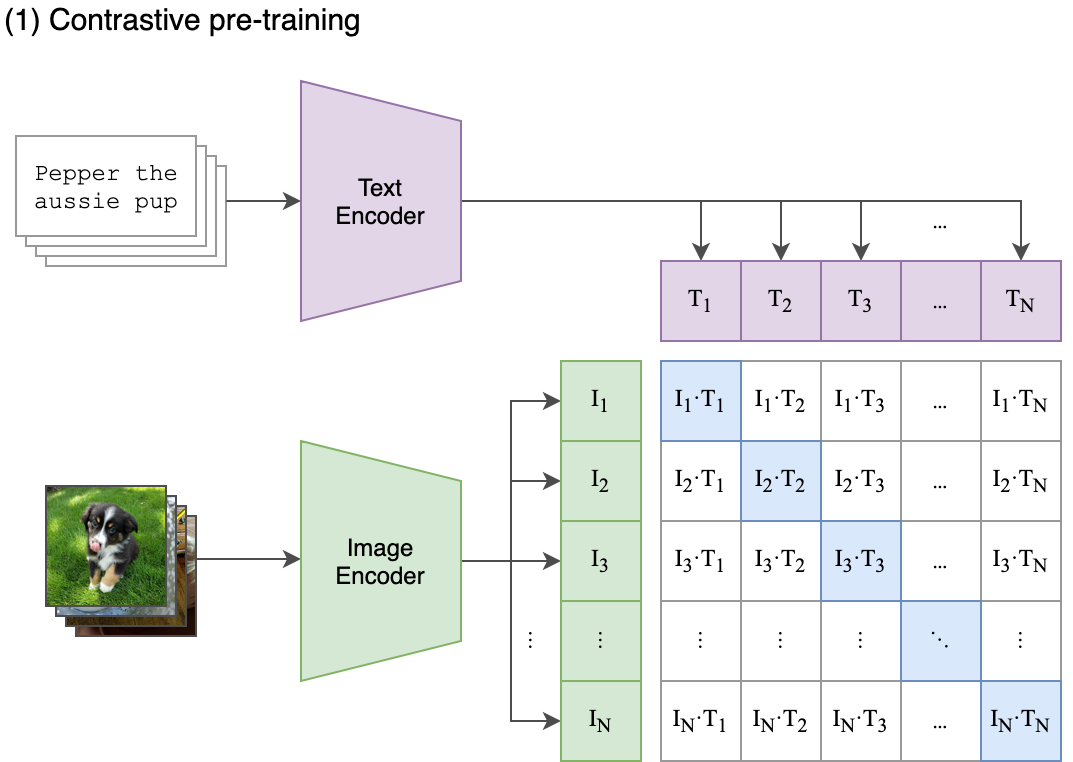
\includegraphics[width=\textwidth]{img/CLIP-structure.png}
    \caption{The CLIP model is composed by two encoders for the two visual and textual data modalities, and employs a contrastive loss function to project the input embeddings into a shared embedding space \cite{radford2021learning}.}
    \label{fig:clip}
\end{figure}


\subsection{Image Encoder}

The \textbf{Image Encoder} in CLIP is tasked with converting an input image into a fixed-dimensional vector that preserves its semantic content. Two main visual backbones were explored by the authors of the original model:

\begin{itemize}
    \item A modified ResNet-50 \cite{he2016deep}, based on improvements from \cite{he2019bag} and \cite{zhang2019making}, which includes changes such as anti-aliasing strided convolutions, attention pooling, and improved normalization techniques;
    \item A Vision Transformer (ViT) \cite{dosovitskiy2020image}, encompassing the ViT-B, ViT-L and ViT-H variants, which divides the input image into a sequence of fixed-size patches, flattens and projects them linearly, adds positional encodings, and processes them via a standard Transformer encoder stack.
\end{itemize}

In both cases, the output is a single vector embedding of size $512$ and normalized to unit length. The ViT version, which has become the most common in the literature relevant to the study conducted in this thesis, operates on $224\times224$ RGB images further split into $32\times32$ patches. A suitable pipeline of transforms is provided to preprocess input images and convert them into this required format. The Transformer encoder is composed of $12$ layers, with $768$ hidden dimensions and $12$ attention heads, followed by a projection head to map the output to $512$ dimensions. The authors have released several checkpoints for models belonging to both the ResNet and the ViT families.
To decide which one to adopt, a careful review was conducted. ViTs have grown in popularity in remote sensing tasks due to their ability to model long-range dependencies and spatial relationships across an image without the locality constraints of convolutional layers. This was demonstrated, among others, by \cite{tuli2021convolutional} who proved the superiority of ViT-B/32 versus ResNet-50 and also its higher consistency with human mistakes; by \cite{dosovitskiy2020image}, who showed how applying the Transformer architecture directly to sequences of images patches would reshape the field of computer vision; multiple other studies confirmed these results \cite{deininger2022comparative}, \cite{hutten2022vision}, \cite{liu2024multivariate}, asserting the superiority of ViTs on CNNs in generalization and making them especially suitable for our case. For these reasons, and based on the most common backbones already tested in the relevant literature, the \emph{ViT-B/32} has been chosen as the go-to architecture for this project and all the reported results are based on it.

\subsection{Text Encoder}

The \textbf{Text Encoder} is a Transformer-based \cite{vaswani2017attention} language model adapted from GPT-like architectures \cite{radford2019language}. It processes a sequence of tokenized input text like class descriptions or full sentences, then encodes the sequence via positional and token embeddings, and forwards it through a $12$-layer transformer with $512$ hidden dimensions and $8$ attention heads. Each input text is truncated or padded to a maximum length of $76$ tokens. A special end-of-text token is used to signal sequence termination, and the final representation of this token is passed through a linear projection head to produce again a $512$-dimensional embedding. This output is likewise normalized to lie on the unit range of values, enabling direct cosine similarity computation and comparison with image embeddings.
Notably, the text encoder is capable of handling free-form natural language input, going beyond the limits of pre-defined class labels. This flexibility is key to CLIP’s zero-shot capabilities, allowing it to reason over arbitrary linguistic prompts and generalize beyond the training distribution.

\begin{comment}  
Both models are optimized during training to encode similar text and image pairs close together in a vector space shared by the two modalities, while also separating the dissimilar pairs. This means that CLIP isn't specifically trained for image classification. It was trained on a huge amount of data from the web, accounting for more than 400 million (image, text) examples; this approach was preferred to adopting an existing dataset mainly because none of them could adequately reflect the natural language variety publicly available on the internet. This dataset was constructed with the goal of covering the broadest possible set of visual concepts, whose corresponding text includes one of $500,000$ queries extracted from Wikipedia and based on word frequency. Then, they made sure there are at least $20,000$ pairs per query. The resulting dataset has a has a similar total word count as the WebText dataset used to train GPT-2. This dataset is known as \textbf{WebImageText (WIT)}.

Understanding natural language makes the model very good across different tasks, and better than traditional CNN models for generalization, and also very good at working with nuanced descriptions with higher level of detail or abstraction. These reasons are what make CLIP's zero-shot performances outstanding and why it's a very interesting model to work with.


(from CLIP's paper) \\

Looking at where zero-shot CLIP notably underperforms we see that zero-shot CLIP is quite weak on several specialized, complex, or abstract tasks such as satellite image classification (EuroSAT and RESISC45), lymph node tumor detection (PatchCamelyon), counting objects in synthetic
scenes (CLEVRCounts), self-driving related tasks such as German traffic sign recognition (GTSRB), recognizing distance to the nearest car (KITTI Distance). These results highlight the poor capability of zero-shot CLIP on more complex tasks. \\

Finally, we found that on satellite image classification datasets it helped to specify that the images were of
this form and we use variants of "a satellite photo
of a {label}."

\end{comment}


\section{Contrastive Learning}

Contrastive Learning is a subfield of Self-Supervised Learning that aims to learn general-purpose representations by distinguishing between similar (positive) and dissimilar (negative) pairs of inputs. It has emerged as a powerful alternative to supervised learning, particularly when large annotated datasets are unavailable, and became a popular approach working at the core of several models in addition to CLIP. In CL, the model is not just trained to predict fixed labels as in standard supervised learning, but to learn embeddings that reflect the semantic similarity between input instances - possibly coming from multiple modalities.
The gist of this mechanism is that models can learn robust features by maximizing the agreement between positive pairs (e.g., an image and its corresponding text description), while minimizing agreement with randomly sampled negative pairs. In this way, CL teaches the model to preserve semantic structure in the learned embedding space without relying on class labels. 
The CLIP model adopts a contrastive learning strategy based on the \emph{Information Noise Contrastive Estimation (InfoNCE) loss}, which was first formalized in \cite{sohn2016improved} and then popularized in \cite{oord2018representation}. This loss function enables the model to meaningfully align image–text pairs in a shared embedding space, ensuring that each image is at the same time close to its true caption and other relevant ones and far from unrelated ones.
Contrastive objectives are designed to maximize the \emph{mutual information} between different views or modalities of the same underlying signal. For instance, image–text pairs or future–past representations in time series may share high-level structure such as object categories, spatial configuration, or narrative content, even if their raw signals differ substantially. Classical losses such as Mean Squared Error (MSE) or Cross-Entropy (CE) do not directly encourage this alignment, actually failing to model abstract relationships.
The InfoNCE objective, instead, addresses this issue by modeling the problem as a slightly modified form of \emph{Noise Contrastive Estimation (NCE)} \cite{gutmann2010noise} \cite{mnih2012fast} \cite{jozefowicz2016exploring}, where the goal is to discriminate a positive pair from a set of negatives. In this formulation, the contrastive task can be thought of as a sort of binary classification problem, where the correct (positive) item must be selected among a pool of candidates.
Following the theoretical framework outlined in by \cite{oord2018representation}, we will now proceed to give a formal definition of the InfoNCE loss. Let $x_{t+k}$ be the future target observation and $c_t$ a context vector representing the past or conditioning signal. Instead of directly modeling the conditional distribution $p(x_{t+k} | c_t)$, which is generally high-dimensional and difficult to treat, CL introduces a scoring function $f_k(x_{t+k}, c_t)$ that is proportional to the ratio of true conditional and marginal distributions:

\begin{equation}\label{f_x}
    f_k(x_{t+k}, c_t) \propto \frac{p(x_{t+k}|c_t)}{p(x_{t+k})}
\end{equation}

This ratio represents the amount of information shared between $x$ and $c$. In practice, $f_k(x, c)$ is parametrized as a log-bilinear function as follows:

\begin{equation}\label{exp}
    f_k(x_{t+k}, c_t) = \exp \left( z^T_{t+k} W_k c_t \right),
\end{equation}

where $z_x$ is the embedding of the target, $c_t$ is the context and $W_k$ is a learned projection matrix. This score is then used in a softmax-like function over a set of $N$ samples where $1$ is a positive sample and $N - 1$ are the negative ones. At this point, let $X = \{x_1, \, x_2, \, \ldots, \, x_N\}$ be a set of samples with one positive instance from $p(x_{t+k} | c_t)$  and the other negatives from $p(x_{t+k})$. The InfoNCe objective to optimize is then defined as:

\begin{equation}\label{InfoNCE}
    \mathcal{L}_N = -\mathbb{E}_X \left[ \log \frac{f_k(x_{t+k}, \, c_t)}{\sum_{x_j \in X} f_k(x_j, c_t)} \right]
\end{equation}

This can be interpreted as the negative log-likelihood of the correct pair under a categorical distribution over all candidates. Therefore, minimizing this loss encourages the model to assign higher scores to true pairs and lower scores to false ones. Importantly, \cite{oord2018representation} show that minimizing InfoNCE corresponds to maximizing a lower bound on the mutual information $I(x;c)$, defined in \ref{I_x}, i.e. the amount of information shared between the input and its context. Thus, the model is not only learning to discriminate but also to capture the shared structure of the paired inputs.

\begin{equation}\label{I_x}
    I(x;c) = \sum_{x, c} p(x, c) \log \frac{p(x|c)}{p(x)}
\end{equation}

During pretraining, CLIP creates an instance discrimination for each batch and optimizes the InfoNCE loss in both directions, image-to-text and text-to-image \cite{radford2021learning} \cite{liu2024remoteclip}. Consider a batch consisting in $N$ (image, text) pairs. The image encoder produces embeddings $\{i_1, \ldots, i_N\}$ and the text encoder embeddings $\{t_1, \ldots, t_N\}$. The similarity matrix $S \in \mathbb{R}^{N \times N}$ is then computed via cosine similarity, i.e. normalized dot product of the embedding vectors:

\begin{equation}\label{sim_matrix}
    S_{ij} = \frac{i_i^Tt_j}{\|i_i\| \| t_j\|}
\end{equation}

CLIP applies then a bidirectional InfoNCE loss for both image-to-text and text-to-image similarities, by computing the cross-entropy over rows and columns of the matrix $S$, with $\tau$ a temperature parameter that scales the logits before applying softmax:

\begin{equation} \label{L_image}
    \mathcal{L_{\text{image}}} = - \frac{1}{N} \sum_{i=1}^N \log \frac{\exp(S_{ii}/\tau)}{\sum_{j=1}^N \exp (S_{ij}/\tau)}
\end{equation}

\begin{equation} \label{L_text}
    \mathcal{L_{\text{text}}} = - \frac{1}{N} \sum_{i=1}^N \log \frac{\exp(S_{ii}/\tau)}{\sum_{j=1}^N \exp (S_{ji}/\tau)}
\end{equation}

A smaller $\tau$ sharpens the distribution, making the model more confident in its predictions. The total loss is then computed as:

\begin{equation}
    \mathcal{L} = \frac{1}{2} (\mathcal{L}_{\text{image}} + \mathcal{L}_{\text{text}})
\end{equation}



\begin{comment}

This is now a categorical cross-entropy of classifying the positive sample correctly, given $\frac{f_k}{\sum_X f_k}$ the prediction output by the model.Optimizing this loss results in the truthful estimation of the density ratio (\ref{f_x}) by $f_k$. In addition, it can be proved that minimizing the InfoNCE Loss $\mathcal{L}_N$ maximizes a lower bound on mutual information. For further details, we remit to the reference paper \cite{oord2018representation}.

The Information Noise Contrastive Estimation (InfoNCE) loss function is a popular method for Self-Supervised Learning (SSL), and specifically Contrastive Learning (CL). In particular, CL aims at teaching the model to distinguish between similar \emph{(positive)} and dissimilar \emph{(negative)} input pairs. This particular loss function then maximizes the alignment between the encodings of positive  input instances


Information Noise Contrastive Estimation (InfoNCE) loss is derived from the framework of noise contrastive estimation. It measures the similarity between positive and negative pairs in the learned embedding space. InfoNCE loss maximizes the agreement between positive pairs and minimizes the agreement between negative pairs.

The key idea behind InfoNCE loss is to treat the contrastive learning problem as a binary classifier. Given a positive pair and a set of negative pairs, the model is trained to discriminate between positive and negative instances. The similarity between instances is measured using a probabilistic approach, such as the softmax function.

InfoNCE loss is commonly used in self-supervised contrastive learning, where positive pairs are created from augmented views of the same instance, and negative pairs are formed using instances from different samples. By optimizing InfoNCE loss, the model learns to capture meaningful similarities and differences in the data points, acquiring powerful representations.


Following the definition provided by \cite{oord2018representation}
One of the most common strategies for unsupervised learning has been to predict future, missing or contextual information.
The main intuition behind our model is to learn the representations that encode the underlying shared
information between different parts of the (high-dimensional) signal. At the same time it discards
low-level information and noise that is more local.
One of the challenges of predicting high-dimensional data is that unimodal losses such as meansquared error and cross-entropy are not very useful, and powerful conditional generative models which
need to reconstruct every detail in the data are usually required. But these models are computationally
intense, and waste capacity at modeling the complex relationships in the data x, often ignoring the
context c.
For example, images may contain thousands of bits of information while the high-level
latent variables such as the class label contain much less information (10 bits for 1,024 categories).
This suggests that modeling p(x|c) directly may not be optimal for the purpose of extracting shared
information between x and c.

When predicting future information we instead encode the target x
(future) and context c (present) into a compact distributed vector representations (via non-linear
2
learned mappings) in a way that maximally preserves the mutual information of the original signals x
and c defined as

\begin{equation}\label{I_x}
    I(x;c) = \sum_{x, c} p(x, c) \log \frac{p(x|c)}{p(x)}
\end{equation}

By maximizing the mutual information between the encoded representations (which is bounded
by the MI between the input signals), we extract the underlying latent variables the inputs have in
common. 

Therefore, $x_t$ are the observations and $c_t$ is the context latent representation. Instead of predicting the future observations $x_{t+k}$ directly with a generative model $p_k(x_{t+k}|c_t)$, a density ratio is modeled to preserve the mutual information between $x_{t+k}$ and ${c_t}$ as follows:

(f formula)

The density $f$ is proportional to the ratio up to a multiplicative constant, and can remain unnormalized as it doesn't need to integrate to $1$. As a positive score, they use a log-bilinear model: 

where $W^T_k c_t$ is a linear transformation used to compute the prediction with a different $W_k$ for every step $k$. Using $f_k$ and inferring $z_{t-+k}$ with an encoder, they circumvent the problem of modeling the high dimensional distribution $x_t$ directly and are able to use samples from the distributions $p(x)$ and $p(x|c)$ without actually evaluating them. At this point, it's possible to apply techniques for parameter estimation like the \emph{Noise Contrastive Estimation (NCE)} \cite{gutmann2010noise} \cite{mnih2012fast} \cite{jozefowicz2016exploring} based on comparing the target value with randomly sampled negative values. Another advantage is that this frameworks keeps its validity for any type of encoder or autoregressive model, whether coming from the audio, vision, language or multimodal domain; due to its great efficiency, it's at the core of many methodologies including SimCLR (Simplified Contrastive Learning of Visual Representations) \cite{chen2020simple} and MoCo (Momentum Contrast) \cite{he2020momentum}, besides CLIP itself \cite{radford2021learning}.

The \emph{InfoNCE Loss} is a function based on NCE and defined as follows: given a set $X = \{x_1, \ldots, x_N\}$ of $N$ random samples containing one positive sample from $p(x_{t+k} | c_t)$ and $N - 1$ negative samples from the "proposal" distribution $p(x_{t+k})$, the objective to optimize is:

\begin{equation}\label{InfoNCE}
    \mathcal{L}_N = -\mathbb{E}_X \left[ \log \frac{f_k(x_{t+k}, \, c_t)}{\sum_{x_j \in X} f_k(x_j, c_t)} \right]
\end{equation}

\end{comment}


\section{Zero-Shot capabilities}

In computer vision, zero-shot learning traditionally refers to the ability to recognize categories that were not seen during training, something that occurs when training and test classes are disjoint \cite{lampert2009learning}. In more recent literature, the definition has expanded to encompass more general forms of transfer learning, where models are evaluated on tasks, categories, or even datasets that are entirely unseen during training.
CLIP introduces an unprecedentedly effective form of zero-shot learning thanks to the robustness of contrastive learning and a large corpus of pretraining image-text pairs. During inference, classification is achieved not only through a conventional softmax over learned weights, but via a nearest-neighbor search in a shared embedding space: images and candidate text prompts are embedded independently, and the most closest pair in the embedding space determines the classification final choice. The procedure of using CLIP as a zero-shot classifier is depicted in Figure \ref{fig:clipzs1}: the text encoder embeds class descriptions based on labels, like
"a photo of a plane", "a photo of a cat", "a photo of a dog" etc. while the image encoder embeds the input image(s). By computing the dot product between the image embedding and all candidate text embeddings, CLIP returns the most semantically appropriate label (in this case, "dog"). 

\begin{figure}[h]
    \centering
    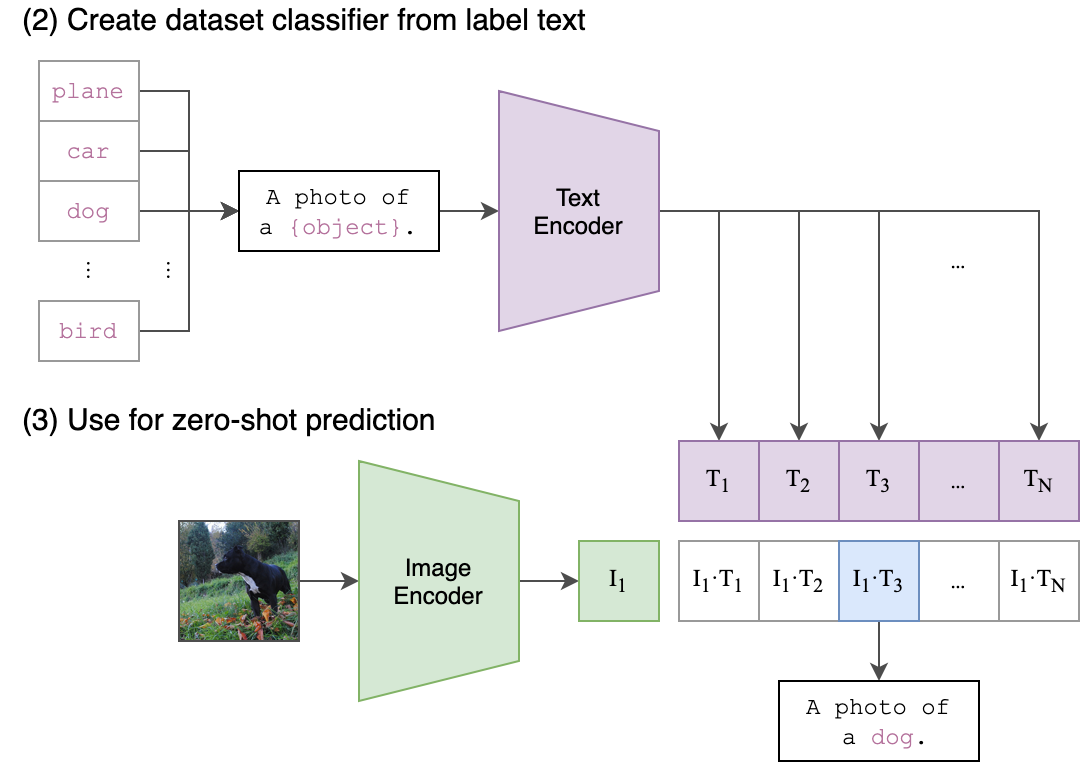
\includegraphics[width=\textwidth]{img/CLIP-zero-shot.png}
    \caption{When using CLIP for zero-shot inference, a user can feed the model custom text and image inputs and obtain similarity scores that quantify how relevant each instance of one modality is to the other.}
    \label{fig:clipzs1}
\end{figure}

This zero-shot transfer ability makes CLIP extremely flexible and represents its true power. Instead of re-training or fine-tuning the model for each new classification task, we can simply prompt it with a set of candidate captions or labels crafted for a specific domain and classify custom input images via similarity matching. This ability has been demonstrated in multiple occasions: Figure \ref{fig:clipzs2} (from the original CLIP paper \cite{radford2021learning}) demonstrated that zero-shot CLIP consistently matches or outperforms fully supervised ResNet-101 models (the state of the art at the time) trained on those very benchmarks in several settings, including highly challenging domain shifts such as sketches (ImageNet-Sketch), renditions (ImageNet-R) and adversarial examples (ImageNet-A), where it improved the trained supervised baseline by $35$, $51$ and $74$ percentage points respectively. These achievements are still among the most impressive in the field.

\begin{figure}[h]
    \centering
    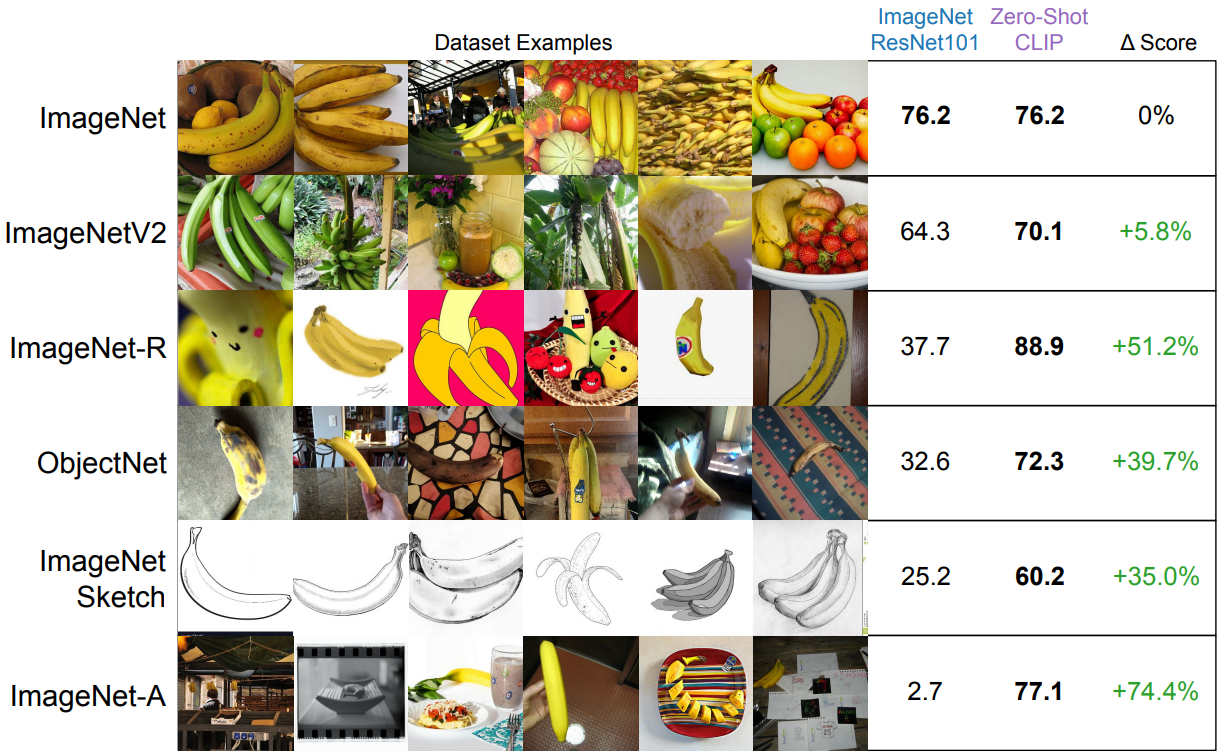
\includegraphics[width=0.7\textwidth]{img/CLIP_zero_shot.png}
    \caption{}
    \label{fig:clipzs2}
\end{figure}

This generalization ability is directly attributable to the scale and diversity of CLIP's pre-training data, as well as its use of natural language supervision. CLIP was trained on a massive proprietary dataset known as \emph{WebImageText (WIT)}, comprising more than $400$ million image–text pairs scraped from the Internet. In an era dominated by social media, there is a massive abundance of data featuring images associated with text in the most disparate domains and language styles. The dataset was built selecting approximately $500,000$ search queries derived from Wikipedia and then ensuring that at least $20,000$ image–text pairs per query were present. Therefore, WIT does not rely on simple class labels, but allows the model to learn from freely occurring captions, descriptions, and alt-text. These naturally occurring annotations are often richer and more descriptive than the labels contained in conventional datasets, capturing both primary and contextual elements within a scene and enabling CLIP to cover a wide range of visual concepts, objects, activities, styles, and scenes.

\begin{comment}
we match the accuracy of the original ResNet-50 on ImageNet zero-shot without needing to use any of the 1.28 million training examples it was trained on.

The zero shot transfer capability of CLIP is what still today makes it an incredibly powerful and robust choice: so much so, that despite being an "old" model (released back in 2021), it's still widely adopted in both research and industry-level technology. 

Zero-shot CLIP is competitive with a fully supervised baseline
\end{comment}


\section{CLIP-like models for Remote Sensing}

\subsection{RemoteCLIP}

The RemoteCLIP model \cite{liu2024remoteclip} is among the first Vision-Language Foundation Models (VLFMs) tailored for Remote Sensing (RS) applications. It is designed to address the challenges of scarce labeled data and semantic alignment in remote sensing by adapting the CLIP paradigm to this domain. Traditional Self-Supervised Learning or Masked Image Modeling-based techniques often fall short in this context due to three main reasons: to begin with, they require large amounts of annotated data for fine-tuning; secondly, they primarily learn low-level features, and are not applicable for retrieval and zero-shot applications, due to the lack of semantic understanding; finally, they have low zero-shot generalization abilities.
The model implements a large-scale, multimodal pretraining framework on a broad and diverse set of image-text pairs, created by merging and augmenting existing RS datasets originally meant for detection, segmentation, and captioning tasks. In this way, RemoteCLIP enables effective transfer to various downstream tasks, including zero-shot classification, linear probing, k-NN classification, image-text retrieval, and object counting.

\begin{figure}[h]
    \centering
    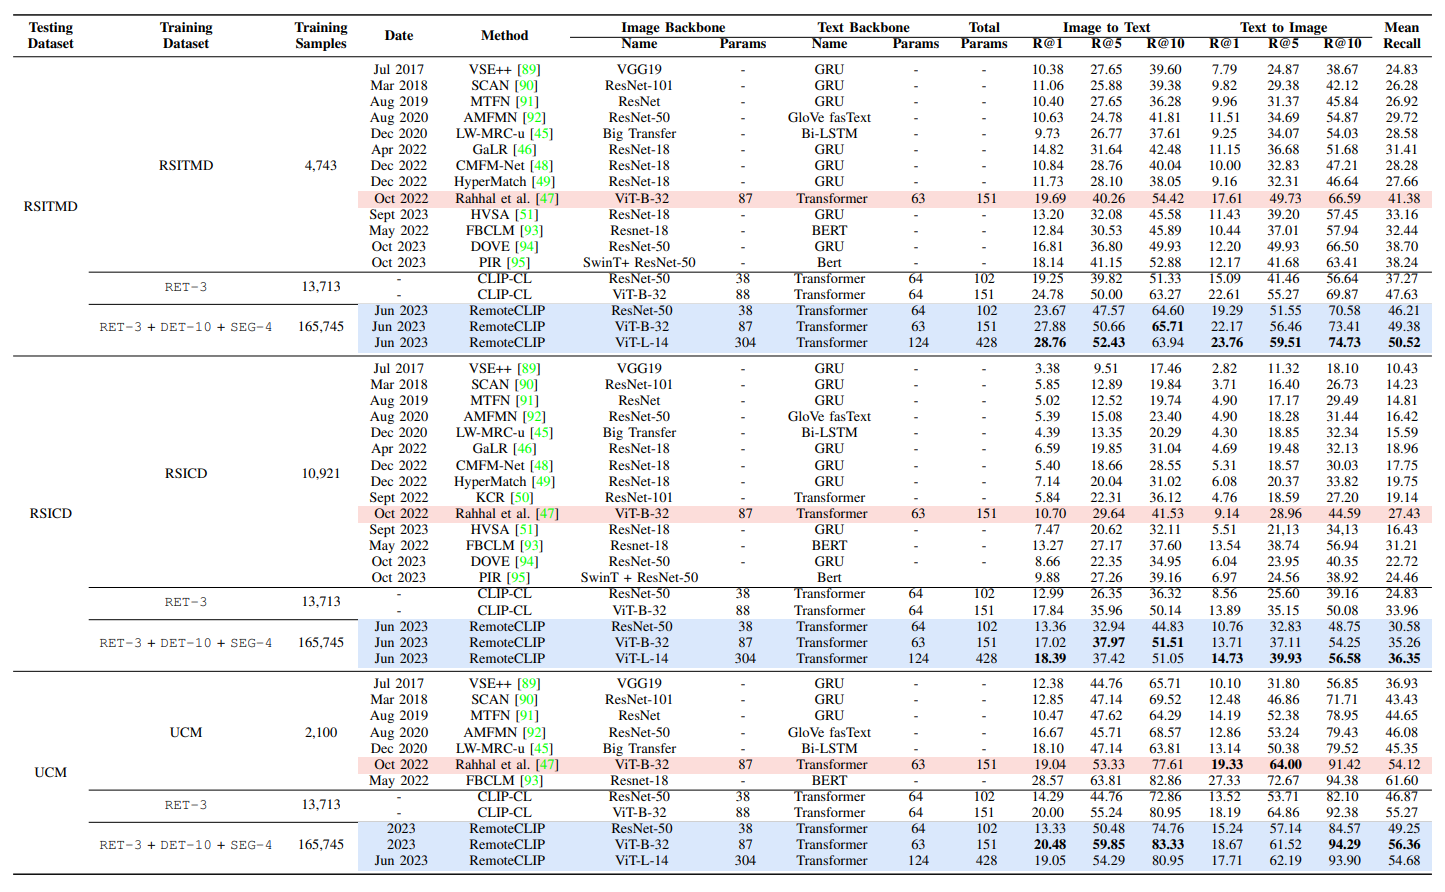
\includegraphics[width=\textwidth]{img/remoteclip-retrieval-performance.png}
    \caption{Cross-modal retrieval results of RemoteCLIP. Previous SOTA are highlighted in red, while RemoteCLIP results are marked in blue.}
    \label{fig:remoteclip-performance}
\end{figure}

To build a considerable pre-training corpus, RemoteCLIP employs two data harmonization techniques:

\begin{itemize}
    \item \emph{Box-to-Caption (B2C)}: generates descriptive captions from object detection datasets using bounding box annotations and class labels;
    \item \emph{Mask-to-Box (M2B)}: converts segmentation annotations into bounding box annotations to expand the pool of usable data.
\end{itemize}
These augmentations result in a dataset approximately $12$ times larger than prior remote sensing captioning corpora. The final training set integrates the following:
\begin{enumerate}
    \item \emph{RET-3}: retrieval data for continual pre-training: three major image-text datasets for Remote Sensing, i.e., RSICD, RSITMD and UCM. These datasets have high caption quality as they were annotated by humans, but a small dataset size;
    \item \emph{DET-10} detection data: major source for dataset expansion including six Remote Sensing datasets with object detection annotations, including DOTA, DIOR, HRRSD, RSOD, LEVIR and HRSC. These datasets have higher resolution and domain diversity than the previous group;
    \item \emph{SEG-4} segmentation data: includes four popular Remote Sensing semantic segmentation datasets, including Vaihingen, Postdam, iSAID and LoveDA..
\end{enumerate}

RemoteCLIP was trained using different Vision Transformer and ResNet backbones of different sizes in the 30-300 millions of parameters range and employs a 12-layer, 8-head Transformer text encoder. Performance on the three most famous RS retrieval benchmarks, evaluated through Recall@K and Mean Recall metrics, shows that RemoteCLIP significantly outperforms existing approaches in both text-to-image and image-to-text scenarios as shown in Figure \ref{fig:remoteclip-performance}), becoming the first strong general-purpose Vision-Language Foundation Model for Remote Sensing.

\subsection{GeoRSCLIP}

Proposed in 2023 concurrently with RemoteCLIP, GeoRSCLIP \cite{zhang2024rs5m} represents a systematic attempt to inject Remote Sensing–specific knowledge into the CLIP framework via a staged domain adaptation paradigm. The authors introduce a general framework for adapting a General Vision-Language Model (GVLM) - pre-trained on general-purpose imagery, like CLIP - to a Domain Vision-Language Model (DVLM) - like GeoRSCLIP - further refined into task-specific models. See Figure \ref{fig:georsclip-framework} for reference.

\begin{figure}[h]
    \centering
    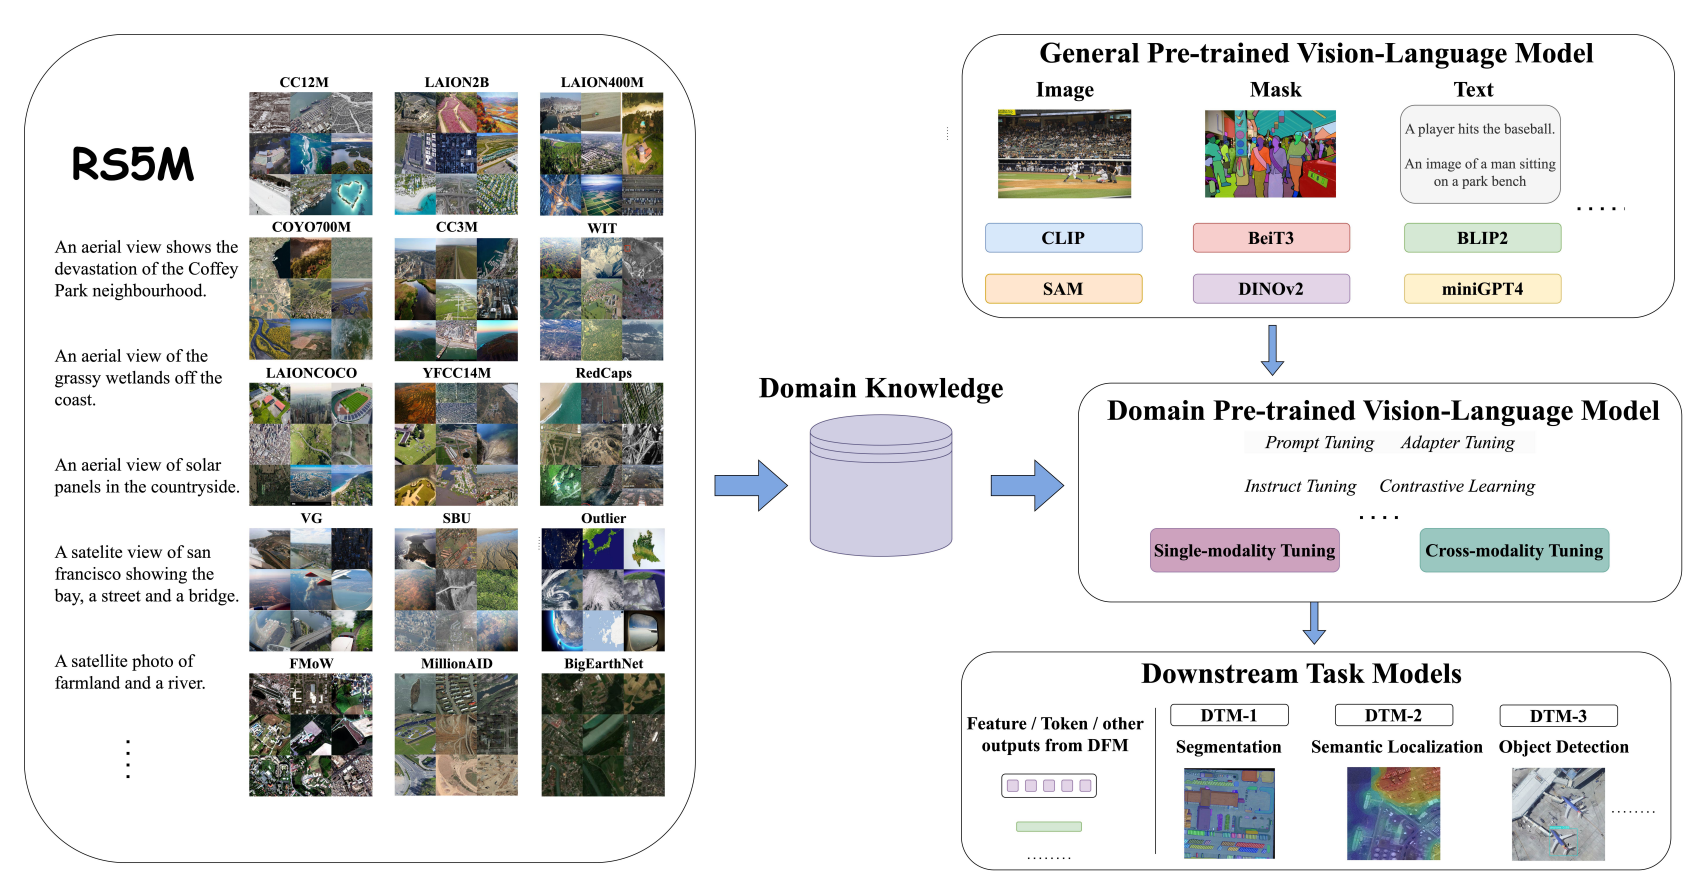
\includegraphics[width=0.75\textwidth]{img/georsclip-framework.png}
    \caption{Illustration of the framework proposed in the GeoRSCLIP paper.}
    \label{fig:georsclip-framework}
\end{figure}

Multiple GeoRSCLIP versions are obtained by fine-tuning CLIP models (ViT-B/32, ViT-L/14, and ViT-H/14) on a newly introduced dataset, RS5M. This large-scale corpus includes 5 million image-text pairs, curated from two major sources:

\begin{itemize}
    \item \textbf{PUB11}: Eleven publicly available general-domain datasets filtered using RS-related keywords, including LAION2B-en, LAION400M, LAIONCOCO, COYO700M, CC3M, CC12M, YFCC15M, WIT, Redcaps, SBU, and Visual Genome. This accounts for 3 million pairs of satellite and aerial images and text;
    \item \textbf{Augmented RS datasets}: Remote Sensing - specific datasets such as BigEarthNet, FMoW, and MillionAID, extended with generated captions obtained by BLIP-2 \cite{li2023blip}.
\end{itemize}

To improve efficiency and enable model reuse, the authors investigate a family of Parameter-Efficient Fine-Tuning (PEFT) methods, including LoRA adapter \cite{hu2021loralowrankadaptationlarge}, Prefix Tuning adapter \cite{li2021prefix}, Pfeiffer adapter \cite{pfeiffer2020adapterfusion}, and UniPELT adapter \cite{mao2021unipelt} (a low-rank-approximated adapter, a prompt-based adapter, a vanilla adapter and a composite adapter). Fine-tuned variants are evaluated on zero-shot classification, cross-modal retrieval, and structured captioning tasks, consistently outperforming RemoteCLIP in reference retrieval scenarios as shown in Figure \ref{fig:georsclip-performance}. The GeoRSCLIP framework exemplifies how targeted domain adaptation, coupled with large-scale pretraining and efficient fine-tuning strategies, can achieve robust multimodal representations for remote sensing cross-modal tasks.

\begin{figure}[h]
    \centering
    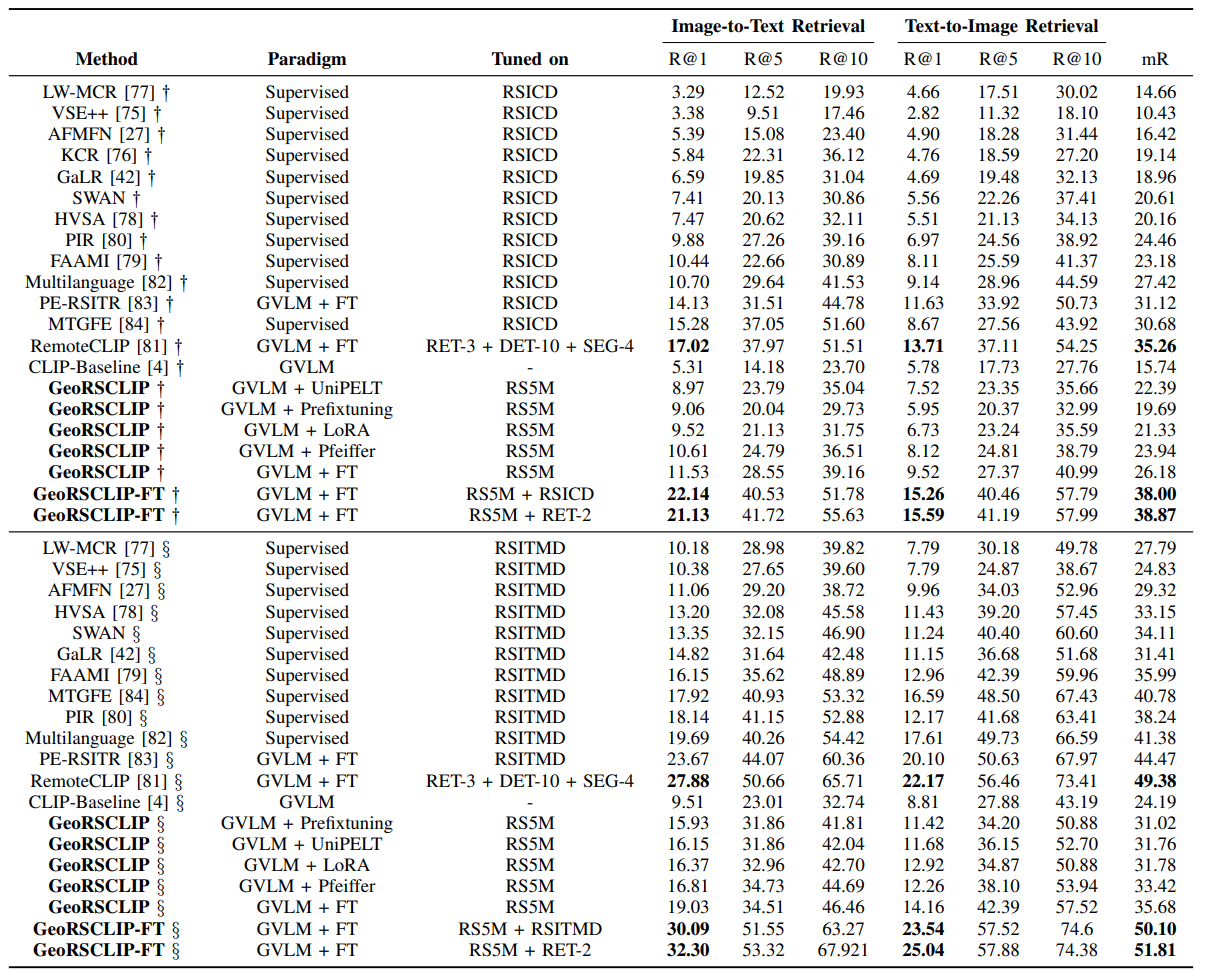
\includegraphics[width=0.8\textwidth]{img/georsclip-retrieval-performance.png}
    \caption{Cross-modal retrieval results for different GeoRSCLIP models trained with R5M. The symbol $\dagger$ means testing on RSICD test dataset, while $\S$means testing on the RSITMD test dataset. Recall@1/5/10 and mean recall are computed. FT stands for Fine Tuning, and the tuning paradigm is specified in the second column.}
    \label{fig:georsclip-performance}
\end{figure}


\subsection{SkyCLIP}

The SkyCLIP model \cite{wang2024skyscript} was released in conjunction to the SkyScript dataset and is the result of CLIP finetuning on it. It was specifically designed to address the challenges of high-altitude and aerial image understanding. SkyScript was designed to address the lack of semantically rich, large-scale image–text collections in them remote sensing domain and together with RS5M \cite{zhang2024rs5m} represents one of the largest datasets available in this field, with its size of $2.6$ million image-text pairs automatically generated and filtered from an initial set of $5.2$ million samples and encompassing over $29,000$ distinct semantic tags. The dataset was constructed by combining high-resolution satellite imagery sampled at various spatial resolutions (from $0.1$m to $30$m GSD, ground sample distance) via Google Earth Engine, with semantic metadata extracted from OpenStreetMap (OSM). Raw OSM tags were then converted into free-form natural language captions and filtered using CLIP-based similarity scoring, retaining the top $30$ to $50\%$ highest quality pairs.

SkyScript is a dataset of comparatively high quality and high resolution images, accompanied by short to medium captions. Continual pretraining of a ViT-B and Vit-L CLIP backbones on this dataset resulted in a model which demonstrated strong zero-shot generalization abilities and overall similar capabilities to GeoRSCLIP, even though the authors didn't include it in evaluation experiments (see Figure \ref{fig:skyclip}). It did outperform CLIP baseline models both general purpose and remote sensing variants, including RemoteCLIP. SkyCLIP demonstrated overall good performances, and even without achieving the state of the art on any specific task or dataset it did surpass several supervised models which were trained directly on the test benchmarks and also improved on the original CLIP. These results highlight the value of the SkyScript dataset for VLM training and finetuning in the context of remote sensing.

\begin{figure}[h]
    \centering
    \subfloat[][]
    {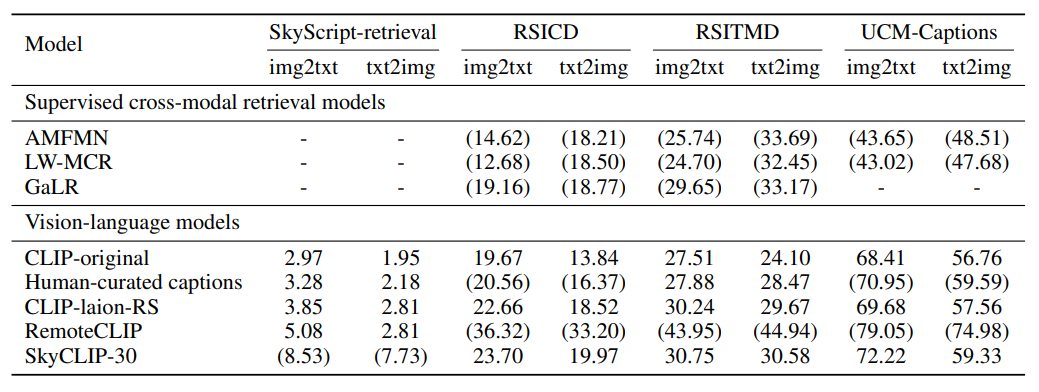
\includegraphics[width=.55\textwidth]{img/skyclip-performances.png} \vspace{0.5cm}} \quad
    \subfloat[][]
    {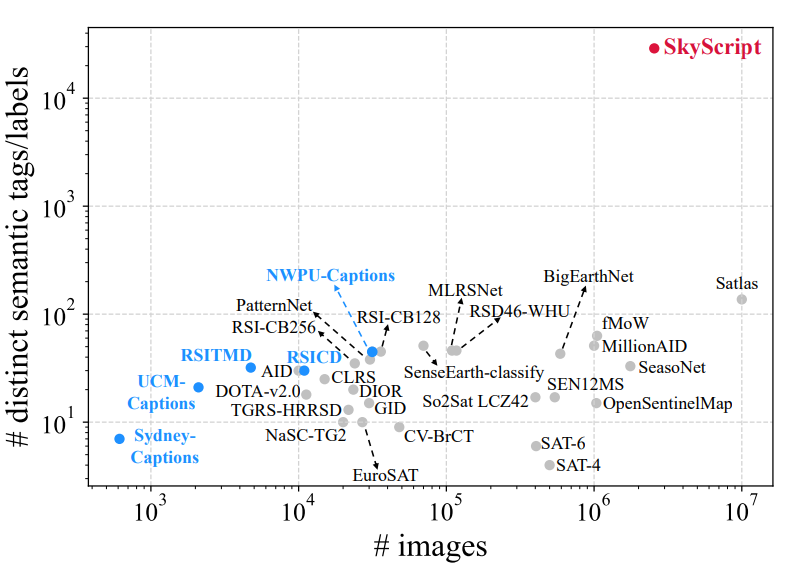
\includegraphics[width=.35\textwidth]{img/skyscript.png}}
\caption{Images taken the the SkyScript original paper \cite{wang2024skyscript}. On the left, mean recall (\%) for benchmark cross-modal retrieval. SkyCLIP-30 is trained on the top $30\%$ SkyScript samples in terms of pairwise similarity. If a dataset is involved in training of a model, then it is bracketed with "()". On the right, a visual comparison of general-purpose RS datasets. Only datasets with $\ge 10,000$ images are shown). SkyScript, is two orders of magnitude more semantically diverse than existing remote sensing image-text datasets.}
\label{fig:skyclip}
\end{figure}


\chapter{Datasets} % ------------------------------------------

\begin{comment}
    A note before proceeding: the following datasets have been adopted due to their nature of benchmark and their importance in the literature, but they are *not* proper image-text datasets (that would be the best option to work with CLIP). This limitation is partly reflected in the final results, but they don't invalidate this work's contribution
\end{comment}

\section{EuroSAT}\label{EuroSAT}

The EuroSAT dataset \cite{helber2019eurosat} is perhaps the most well known and widely used benchmark in the remote sensing field for land use and land cover (LULC) classification. It is built upon the freely available collections of multispectral Sentinel-2 satellite imagery from ESA’s Copernicus program, and was explicitly designed to support research in Earth Observation using modern deep learning methods. In this thesis, EuroSAT has been used extensively: it served as a prototyping environment for model testing, exploration of normalization strategies and model training, representing the main reference point to contextualize the performance on other datasets. While EuroSAT is smaller and less diverse than more recent benchmarks (including but not limited to GEO-Bench \cite{lacoste2023geo}) it remains a critical resource thanks to its long-standing use in the literature, high accessibility and usability, and simple structure. EuroSAT consists of $27,000$ labeled and geo-referenced image patches, each measuring 64×64 pixels and captured across $13$ spectral bands by the Sentinel-2 satellite constellation. The dataset spans $10$ land use and land cover classes, carefully selected for their visibility at $10$m spatial resolution and prevalence across Europe: \emph{Annual Crop}, \emph{Permanent Crop}, \emph{Pasture}, \emph{Forest}, \emph{Herbaceous Vegetation}, \emph{Highway}, \emph{Residential Buildings}, \emph{Industrial Buildings}, \emph{River}, \emph{Sea/Lake}. Each class contains between $2,000$ and $3,000$ image samples, as evenly distributed as possible to avoid class imbalance. A handful of EuroSAT images spanning across all present labels is shown in Figure \ref{fig:eurosatgrid}, while a summary of the dataset characteristics is provided in Table \ref{tab:euclasstypes}. In order to ensure geographical diversity and seasonal variability, the patches were extracted from satellite scenes over the 34 European countries covered in the European Urban Atlas and specifically: Austria, Belarus, Belgium, Bulgaria, Cyprus, Czech Republic (Czechia), Denmark, Estonia, Finland, France, Germany, Greece, Hungary, Iceland, Ireland, Italy / Vatican City, Latvia, Lithuania, Luxembourg, Macedonia, Malta, Republic of Moldova, Netherlands, Norway, Poland, Portugal, Romania, Slovakia, Slovenia, Spain, Sweden, Switzerland, Ukraine and United Kingdom. An extra effort was put into excluding cloud-covered or visually corrupted samples and all the images have all been manually checked. The labels selection process tried to emphasized both inter- and intra-class diversity, as much as it could be captured at the given resolution: for example, the label "Forest" doesn't differentiate between coniferous or broadleaf types of woods, while "Industrial Buildings" and "Residential Buildings" are considered much more easy to distinguish at this level of visibility. The EuroSAT dataset was released in two versions, an RGB-only and an MSI one: they only differ in the amount of image data made available.

\begin{wrapfloat}{figure}{I}{0pt} % I inner margin, O outer margin
    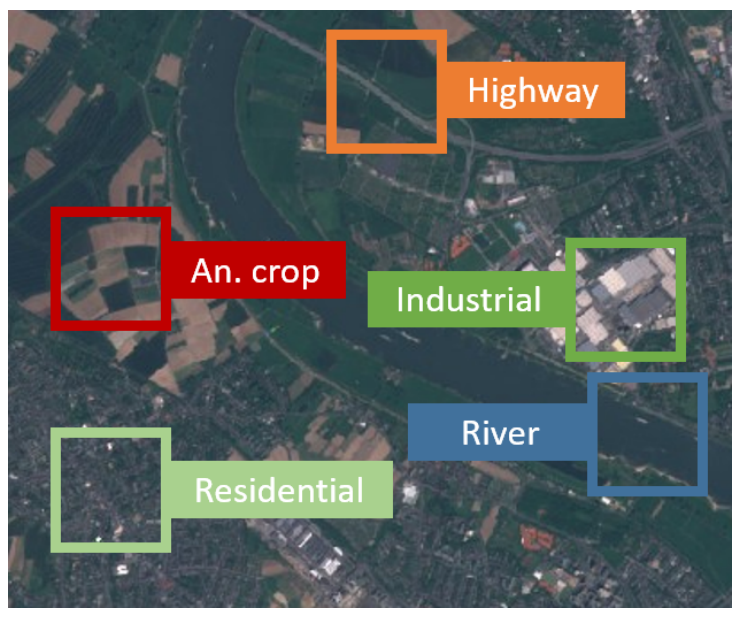
\includegraphics[width=0.4\textwidth]{img/EuroSAT_paper.png}
    \caption{Example taken from \cite{helber2019eurosat} showing different Sentinel-2 based image patches extracted to identify different land use and land cover classes in the EuroSAT dataset.}
    \vspace{-0.7cm}
\label{fig:eurosatpatch}
\end{wrapfloat}

In this thesis, we used both: the former for RGB performance baselines and the latter for MSI model training, respectively. EuroSAT MSI is a dataset rich in multispectral information, accounting for 13 total bands captured by Sentinel-2's optical sensors for each image. They cover the visible (RGB), near-infrared (NIR), red edge, and short-wave infrared (SWIR) regions of the electromagnetic spectrum as described in detail in Table \ref{tab:sentinel2_bands}. This makes EuroSAT an ideal candidate for developing and evaluating models that leverage information beyond the standard RGB channels.
EuroSAT patches were collected by sampling cloud-free Sentinel-2 tiles over urban and rural areas included in the European Urban Atlas. The selection process emphasized intra-class diversity by sampling across seasons and regions. For example, the “Forest” class includes both coniferous and broadleaf types, while “Industrial Buildings” and “Residential Buildings” are derived from urban fabric classes in the Atlas mapping guide. All images are georeferenced, allowing spatial correlation with GIS layers. The dataset was released in a patch-based form to simplify training and evaluation for classification and retrieval models that, as a matter of fact, have been widely using EuroSAT for the great support it provides to supervised land cover classification with standard ML/DL pipelines, benchmarking of zero-shot and multimodal models and exploration of multispectral embeddings and band-wise information gain.

\vspace{0.5cm}

\begin{figure}[h]
    \centering
    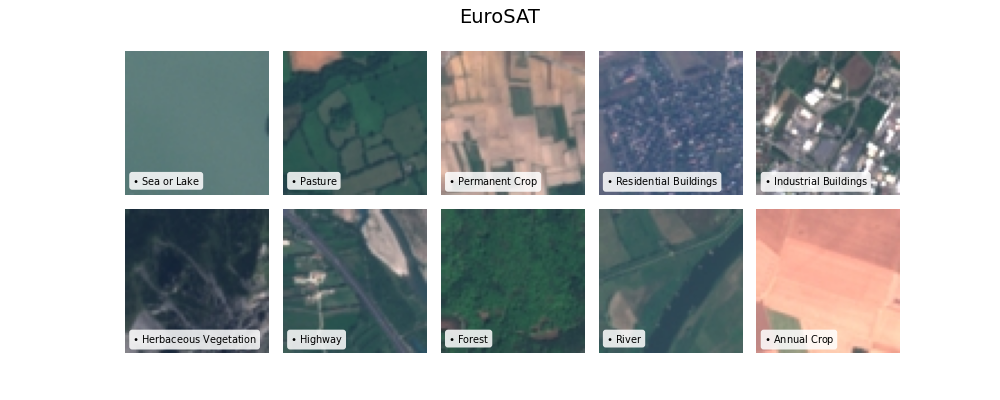
\includegraphics[width=\textwidth]{img/EuroSAT_image_grid.png}
    \caption{Sample images from the 10 classes contained in the EuroSAT original dataset.}
    \label{fig:eurosatgrid}
\end{figure}


\begin{table}[ht]
\centering
\footnotesize
\renewcommand{\arraystretch}{1.2}
    \begin{tabular}{rcccccclcl}
    \toprule
    Name & Image Size & \# Classes & Train & Val & Test & \# Bands & RGB res & Sensors  \\
    \midrule
    EuroSAT & 64 $\times$ 64 & 10 & 10000 & 5000 & 5000 & 13 & 10.0m & Sentinel-2 \\
    \bottomrule
    \end{tabular}
\vspace{0.3cm}
\caption{\normalsize Summary of EuroSAT characteristics.}
\label{tab:euclasstypes}
\end{table}


\begin{table}[ht]
\centering
\scriptsize
    \begin{tabular}{lccl}
    \toprule
    \textbf{Band Name} & \textbf{Resolution} & \textbf{Wavelength} & \textbf{Primary Use} \\
    \midrule
    B01 - Aerosols & 60 m & 443 nm & Atmospheric correction, aerosol detection \\
    B02 - Blue & 10 m & 490 nm & Vegetation/water analysis, true-color composites \\
    B03 - Green & 10 m & 560 nm & Chlorophyll reflectance, plant health \\
    B04 - Red & 10 m & 665 nm & NDVI, land cover discrimination \\
    B05 - Red Edge 1 & 20 m & 705 nm & Chlorophyll concentration \\
    B06 - Red Edge 2 & 20 m & 740 nm & Crop vigor, plant stress \\
    B07 - Red Edge 3 & 20 m & 783 nm & Canopy structure, precision agriculture \\
    B08 - NIR & 10 m & 842 nm & Biomass estimation, NDVI \\
    B08A - Red Edge 4 & 20 m & 865 nm  & Gap-filling between red edge and NIR \\
    B09 - Water Vapor & 60 m & 945 nm & Atmospheric humidity \\
    B10 - Cirrus & 60 m & 1375 nm & Cirrus cloud detection \\
    B11 - SWIR 1 & 20 m & 1610 nm & Soil moisture, burned area detection \\
    B12 - SWIR 2 & 20 m & 2190 nm & Mineral/soil mapping, snow cover \\
    \bottomrule
    \end{tabular}
\vspace{0.3cm}
\caption{\normalsize EuroSAT MSI bands provided by Sentinel-2, along with spatial resolution, central wavelength, and descriptive use cases.}
\label{tab:sentinel2_bands}
\end{table}


\begin{comment}
\begin{table}[ht]
\centering
\scriptsize
%\renewcommand{\arraystretch}{1.2}
\begin{tabular}{lccp{6cm}}  % last column for description
\toprule
\textbf{Band Name} & \textbf{Spatial} & \textbf{Central} & \textbf{Description} \\
{} & \textbf{Resolution} & \textbf{Wavelength} & \\
{} & \emph{m} & \emph{nm} & \\
\midrule
B01 - Aerosols  & 60 & 443  & Useful for atmospheric corrections and aerosol detection. \\
B02 - Blue & 10 & 490  & Penetrates water; useful for bathymetry, atmospheric corrections, and distinguishing vegetation. \\
B03 - Green & 10 & 560  & Sensitive to plant reflectance; useful for vegetation analysis and true color imagery. \\
B04 - Red & 10 & 665  & Captures vegetation and urban features; key in NDVI computation. \\
B05 - Red edge 1 & 20 & 705  & Useful for analyzing chlorophyll content and vegetation stress. \\
B06 - Red edge 2 & 20 & 740  & Enhanced vegetation sensitivity; used in crop monitoring. \\
B07 - Red edge 3 & 20 & 783  & Helps assess canopy structure and plant health. \\
B08 - NIR & 10 & 842  & Strong vegetation reflectance; essential in NDVI and biomass analysis. \\
B08A - Red edge 4 & 20 & 865  & Fills spectral gap between NIR and red edge; aids precision agriculture. \\
B09 - Water vapor & 60 & 945  & Targets atmospheric water vapor content; useful in climate and humidity studies. \\
B10 - Cirrus & 60 & 1375 & Detects high-altitude cirrus clouds; supports cloud masking. \\
B11 - SWIR 1 & 20 & 1610 & Used for vegetation moisture, snow, and burn area mapping. \\
B12 - SWIR 2 & 20 & 2190 & Helps in soil and mineral discrimination, snow and fire monitoring. \\
\bottomrule
\end{tabular}
\vspace{0.3cm}
\caption{Sentinel-2 MSI spectral bands with spatial resolution, central wavelength, and descriptive use cases.}
\label{tab:sentinel2_bands}
\end{table}
\end{comment}



\section{GEO-Bench}

The GEO-Bench dataset suite \cite{lacoste2023geo} was introduced in 2023 with the goal of promoting the evaluation of general-purpose models on Earth Observation data. Its aim is to provide a comprehensive and unified framework for benchmarking large-scale models, either vision-only or vision-language, across multiple geospatial tasks, sensors, and input typology. To this purpose, the benchmark combines data from a variety of Earth Observation satellite missions and sources, focusing on both practical diversity and scientific relevance, and ensuring global geographical coverage as shown in Figure \ref{fig:geoworld}. GEO-Bench comprises 12 total datasets:
\begin{itemize}
    \item 6 dedicated to classification tasks;
    \item 6 dedicated to segmentation tasks.
\end{itemize}
In this work, we exclusively focus on the \emph{classification} datasets, which encompass a rich set of tasks including binary, multiclass, and multilabel classification. Detailed characteristics are presented in Table \ref{fig:geoinfo} and Table \ref{tab:geoclasstypes}. These six datasets are:
\begin{itemize}
    \item \textbf{m-brick-kiln}: binary classification (detecting presence of brick kilns, originally introduced in \cite{lee2021scalable});
    \item \textbf{m-pv4ger}: binary classification (detecting presence of rooftop solar panels, originally presented in \cite{mayer20223d});
    \item \textbf{m-forestnet}: multiclass classification (identify deforestation drivers, firstly appearing in \cite{irvin2020forestnet});
    \item \textbf{m-eurosat}: multiclass classification (identify land use and cover with deep learning methods, presented in \cite{helber2019eurosat});
    \item \textbf{m-so2sat}: multiclass classification (idenfity local climate zones, originally introduced in  \cite{zhu2019so2sat});
    \item \textbf{m-bigearthnet}: multilabel classification (identify relevant land cover phrases, proposed by \cite{sumbul2021bigearthnet}).
\end{itemize}
Each dataset originates from independent research projects and applications, and they vary significantly in terms of image resolution, class structure, geographic coverage, and number of spectral bands used. Then, they were randomly sampled and uniformly preprocessed to guarantee a unified source of data in the benchmark. Since datasets are "modified", their names were prepended with a starting "m-" to distinguish them from the original version.


\begin{figure}[h]
    \centering
    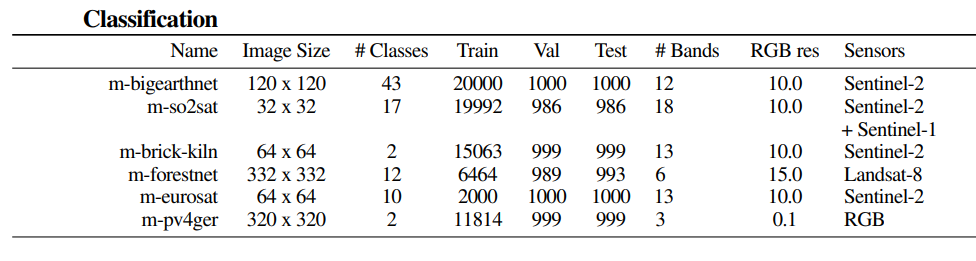
\includegraphics[width=\textwidth]{img/geobench-datasets-classification-info-cut.png}
    \caption{Characteristics of datasets in the benchmark \cite{lacoste2023geo}.}
    \label{fig:geoinfo}
\end{figure}


\vspace{-0.5cm}
\paragraph{Multispectral Properties}

One of the main strengths of GEO-Bench, and the main reason why it was chosen for this work, lies in its extensive use of multispectral and multi-sensor data. Each dataset contains satellite imagery processed from sources such as the Sentinel-1, Sentinel-2, and Landsat 8 constellations, including a total amount of spectral bands that ranges from 3 and 18. These bands go beyond RGB visible light and span through near-infrared (NIR), short-wave infrared (SWIR), red edge, and specialized atmospheric channels. This makes GEO-Bench especially relevant for testing the generalization capacity of models over multispectral data. The fundamental properties of the MSI channels are general, as they only depend on the sensor, and below we report a brief summary. For more details, see Table \ref{tab:sentinel2_bands}.
\begin{itemize}
    \item RGB (B02–B04): used for standard visual interpretation and land classification;
    \item Red Edge (B05–B08A): useful for crop monitoring and vegetation health analysis;
    \item NIR (B08): used for biomass estimation and vegetation indexes;
    \item SWIR (B11–B12): applied for burn area mapping and mineral detection;
    \item Water vapor and cirrus (B09–B10): used for atmospheric analysis and structure detection.
\end{itemize}

\paragraph{Diversity of tasks}

In terms of machine learning paradigms, the classification datasets are designed for the following tasks:
\begin{enumerate}[i)]
    \item Binary Classification: distinguishing between two binary outcomes, e.g. detection of a specific element in an image (m-brick-kiln, m-pv4ger);
    \item Multiclass Classification: selecting one class that best describes the images from multiple mutually exclusive options (m-forestnet, m-eurosat, m-so2sat);
    \item Multilabel Classification:selecting multiple non-exclusive labels that are relevant for each image (m-bigearthnet). This is a more complex task and typically leveraged in scenarios where the focus is on the whole content of an image rather than on a specific object, like image-to-text retrieval and image understanding or captioning. 
\end{enumerate}
Given the nature of CLIP-based models, label predictions are extracted based on the similarity computed by the model between the image and the labels embeddings; the multilabel setting requires a different approach, as we explain in detail in a following section.


\begin{figure}[h]
    \centering
    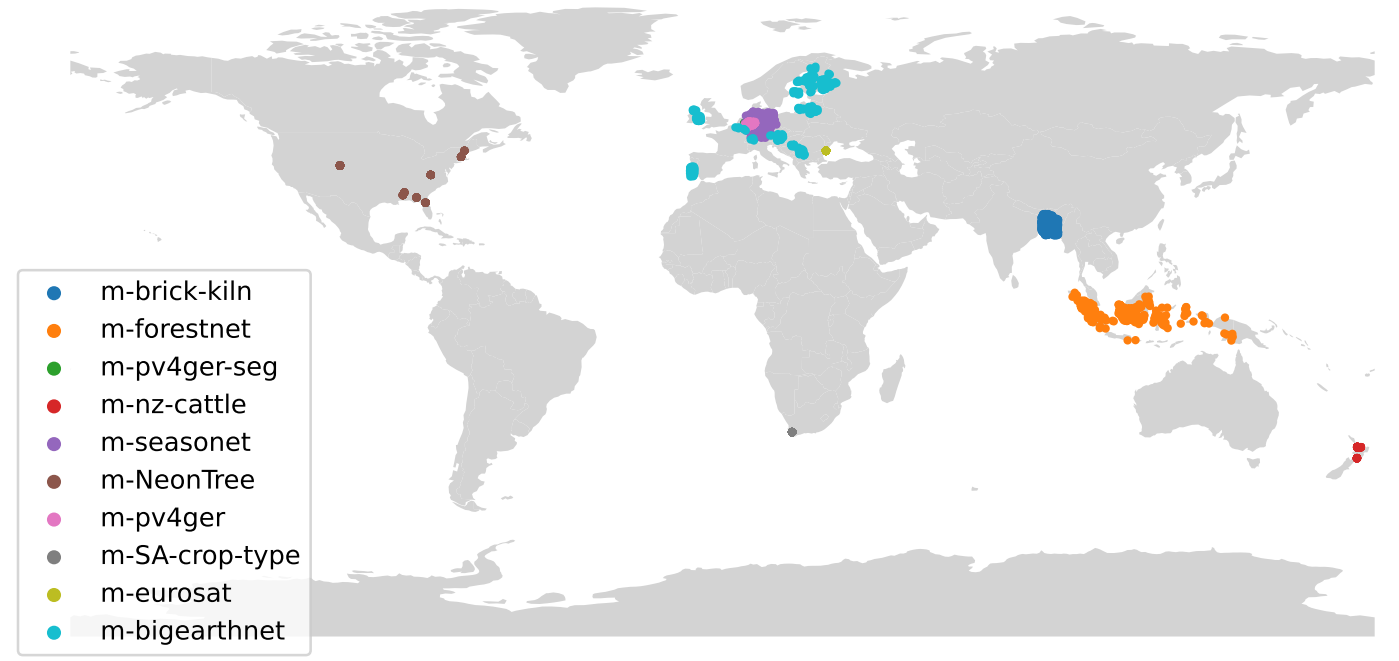
\includegraphics[width=0.6\textwidth]{img/geobench_world_coverage.png}
    \caption{The world coverage of different datasets of the benchmark, as reported in \cite{lacoste2023geo}.}
    \label{fig:geoworld}
\end{figure}  


\begin{table}[ht]
\centering
\footnotesize
\renewcommand{\arraystretch}{1.2}
    \begin{tabular}{lcccc}
    \toprule
    \textbf{Dataset} & \textbf{Origin} & \textbf{Classification task} & \textbf{\# Classes} & \textbf{Type of classes}  \\
    \midrule
    m-brick-kiln & GEO-Bench & binary & 2 & short captions \\
    m-pv4ger & GEO-Bench & binary & 2 & short captions \\
    m-forestnet & GEO-Bench & multiclass & 12 & words \\
    m-eurosat & GEO-Bench & multiclass & 10 & words \\
    m-so2sat & GEO-Bench & multiclass & 17 & words \\
    m-bigearthnet & GEO-Bench & multilabel & 43 & captions \\
    \bottomrule
    \end{tabular}
\vspace{0.3cm}
\caption{\normalsize Classification task details for every dataset analyzed.}
\label{tab:geoclasstypes}
\end{table}

\subsection{m-brick-kiln}

The m-brick-kiln dataset is a binary classification dataset curated to support the detection of brick kilns: a "kiln" is a kind of furnace where brick are "baked". Brick kilns are small scale industrial structures known for their high pollution levels, especially prevalent across South Asia and representing a significant source of carbon emissions and air pollution. Monitoring their presence and compliance with environmental regulations is a key step in addressing the environmental challenges posed by informal and unregulated industrial activity.
The original work that inspired this dataset focused on the accurate study about identification of illegal brick kilns across Bangladesh using high-resolution imagery and machine learning models \cite{lee2021scalable}. However, due to the proprietary nature of the original data, GEO-Bench offers a public alternative by replacing the input modality with Sentinel-2 imagery acquired via Google Earth Engine, maintaining alignment with the original study’s ground truth annotations.
The dataset contains image patches with size of 64$\times64$ pixels and spanning across 13 spectral bands (B01 through B12, excluding B10 due to preprocessing), with each patch labeled as either:

\begin{itemize}
    \item $1$: not brick kiln (no brick kiln is present);
    \item $0$: brick kiln (a brick kiln is present);
\end{itemize}

\vspace{-0.3cm}

\begin{figure}[h]
    \centering
    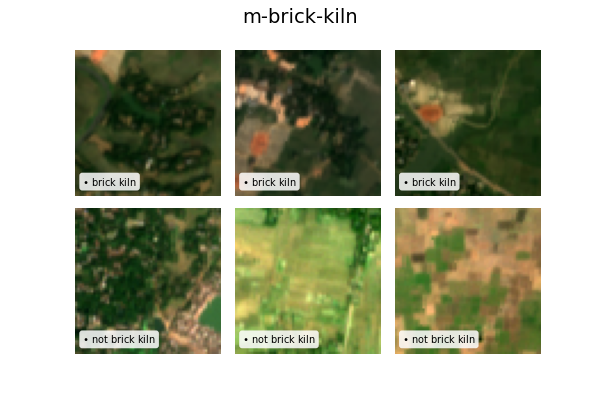
\includegraphics[width=0.7\textwidth]{img/m-brick-kiln_image_grid.png}
    \vspace{-0.5cm}
    \caption{\normalsize Sample images from the 2 classes contained in the m-brick-kiln dataset from GEO-Bench.}
    \label{fig:brickgrid}
\end{figure}

Multiple image samples from both classes are shown in Figure \ref{fig:brickgrid}, to give an idea of what brick kilns look like from a satellite perspective and how they differ from images that do not contain any. The image patches are extracted from the time window between October 2018 and May 2019, matching the observation period of the original kiln location survey. The derived subset provided by GEO-Bench includes $17,061$ following official splits in train, validation and test sets while preserving class proportions. All patches are stored in HDF5 format with metadata including geolocation bounds and class labels.
This dataset represents a practical and non-trivial binary classification task, given the medium-low resolution of the images. That's why it is highly relevant for testing fine grained detection capacity in VLMs like CLIP. Additionally, the inclusion of all 13 Sentinel-2 bands makes it ideal to test and compare model performances on different multispectral input.


\subsection{m-pv4ger}

The m-pv4ger dataset is another binary classification benchmark designed to identify the presence of photovoltaic (PV) systems on rooftops relying on satellite imagery. The task is of significant relevance to energy infrastructure monitoring and sustainability planning, as solar PV installations are increasingly deployed at residential and industrial scales. However, due to their highly decentralized and small-scale nature, PV systems are difficult to track with traditional inventory methods. Therefore, in the original work associated with this dataset the authors introduced a 3D-PV-Locator \cite{mayer20223d}, a hybrid approach combining aerial imagery and 3D building data to estimate both the position and orientation (azimuth and tilt) of PV systems across Germany. While the full 3D pipeline involves complex processing steps, the GEO-Bench version simplifies this to a yes/no classification task: detecting whether or not a PV system is present in the given image patch. The dataset includes $320\times 320$ Sentinel-2 image patches annotated as follows:

\begin{itemize}
    \item $1$: no solar panel (no solar panel is present);
    \item $0$: solar panel (a solar panel is present);
\end{itemize}

\vspace{-0.3cm}

\begin{figure}[h]
    \centering
    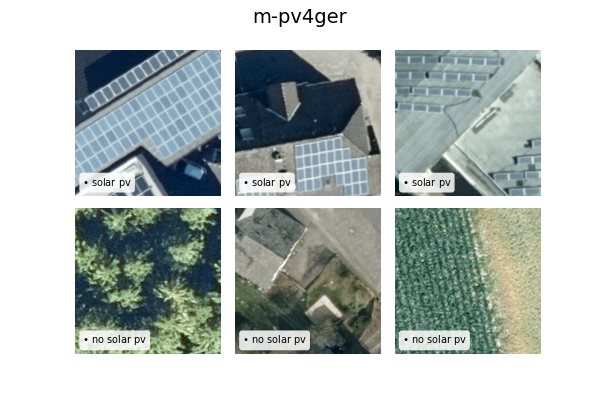
\includegraphics[width=0.7\textwidth]{img/m-pv4ger_image_grid.png}
    \vspace{-0.5cm}
    \caption{\normalsize Sample images from the 2 classes contained in the m-pv4ger dataset from GEO-Bench.}
    \label{fig:solargrid}
\end{figure}

Multiple image samples from both classes are shown in Figure \ref{fig:brickgrid} for visual reference. It's important to highlight that m-pv4ger is a \emph{RGB-only} dataset, an isolated case in the whole GEO-bench collection, where only the three Reg, Green and Blue bands are provided. To ensure accurate annotations, all original imagery was collected over the regions of Germany and the positive samples were matched to the national solar panel registry. The dataset version found in GEO-Bench accounts for $13,812$ images split into training, validation, and test subsets, again preserving class balance across all splits.
Compared to m-brick-kiln, the visual cues that define PV systems are easier to detect given the overall higher resolution of the image data. For its characteristics, m-pv4ger brings great diversity to GEO-Bench and represents a relevant use-case for practical applications in energy forecasting, smart grid planning, and green infrastructure monitoring, strengthening its utility in broader EO model evaluation frameworks.


\subsection{m-forestnet}

The m-forestnet dataset tackles a more subtle and complex classification task: identifying the main direct drivers of primary forest loss in tropical regions, with a particular focus on Indonesia. Forest loss is a major contributor to global greenhouse gas emissions and loss of biodiversity, and understanding its most common underlying causes is critical for designing effective conservation and land use policies.
Originally developed in the ForestNet study by Irvin et al. \cite{irvin2020forestnet}, the dataset consists of Landsat-8 satellite imagery paired with expert-annotated labels that identify the primary driver of forest degradation in each image patch. These drivers span both natural and anthropogenic categories and include activities such as plantation expansion, smallholder agriculture, mining, infrastructure development, and wildfires.
In GEO-Bench, this dataset has been adapted to a multiclass classification problem with 12 classes, each one corresponding to a unique cause of deforestation. The task is notably challenging to tackle with general-purpose VLMs, due to its high specificity and the striking resemblance of the images at a first glance. The GEO-Bench dataset version consists of $8,446$ image patches centered around a region of forest loss, delimited by contours as shown in Figure \ref{fig:forestnetgrid}. Each patch has size $332 \times 332$, the highest image quality of the benchmark, drawn from multispectral imagery with $6$ available bands determined by the Landsat-8 sensor configuration. These are generally mismatched from the ones provided by Sentinel-2, therefore special attention was given to re-ordering the multispectral channels before passing the images to our models, as described in following sections.
The inclusion of m-forestnet in GEO-Bench adds important semantic depth and increased task complexity to the benchmark. Here the model needs to be able to distinguish fine-grained and high-level land use patterns, in images apparently very similar to each other.

\vspace{0.3cm}

\begin{figure}[h]
    \centering
    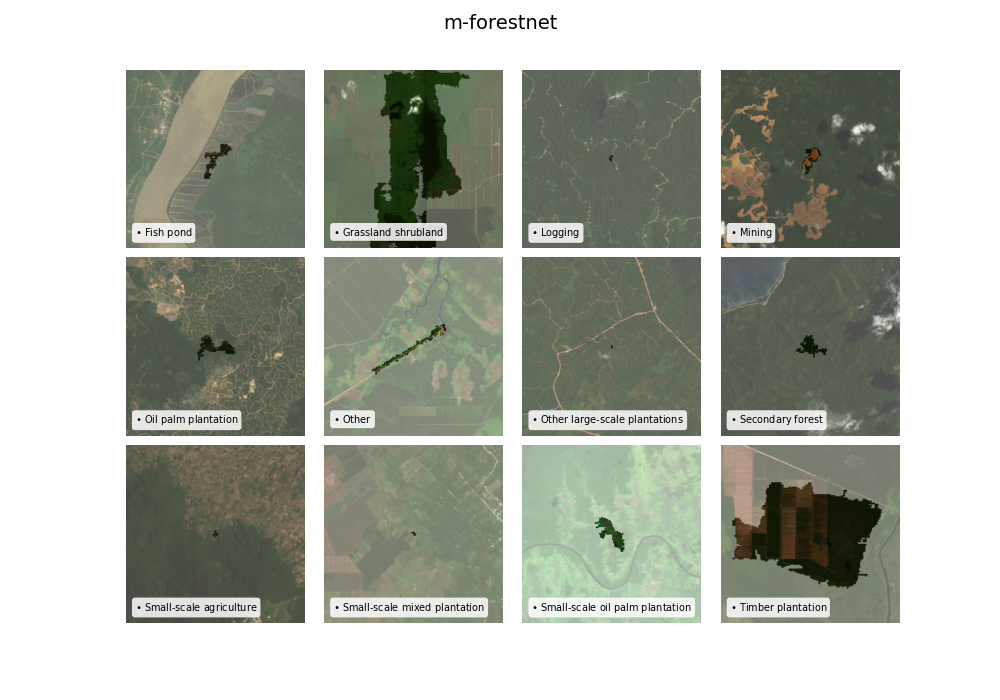
\includegraphics[width=0.8\textwidth]{img/m-forestnet_image_grid.png}
    \caption{\normalsize Sample images from the 12 classes contained in the m-forestnet dataset from GEO-Bench.}
    \label{fig:forestnetgrid}
\end{figure}


\subsection{m-eurosat}

The m-eurosat dataset is a multispectral adaptation of the well-known EuroSAT dataset \cite{helber2019eurosat} described in the previous section \ref{EuroSAT}. Originally designed for land use and land cover classification based on Sentinel-2 imagery, the GEO-Bench version features the same 10 mutually exclusive land cover classes and has been adapted to follow the standardized format of the benchmark. The image patches have still size $64 \times 64$ and have been selected in a subset of $4,000$ samples, always ensuring class balance. Compared to the original EuroSAT, this version features standardizes data formatting to conform to GEO-Bench's unified structure and stored in HDF5 format to encode labels and task metadata along with the images. While not substantially changing the input data or labels with respect to the original dataset, m-eurosat contributes to the robustness of GEO-Bench and plays a useful role to evaluate models on a comprehensive set of applications, in addition to enabling direct comparisons with earlier literature that used the original dataset. The reader can get a glimpse of m-eurosat samples in Figure \ref{fig:meurosatgrid}.


\begin{figure}[h]
    \centering
    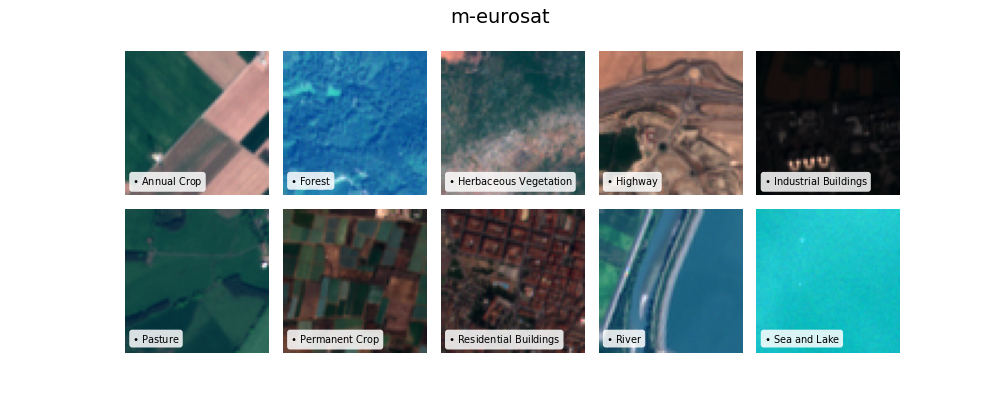
\includegraphics[width=\textwidth]{img/m-eurosat_image_grid.png}
    \caption{\normalsize Sample images from the 10 classes contained in the m-eurosat dataset from GEO-Bench.}
    \label{fig:meurosatgrid}
\end{figure}


\subsection{m-so2sat}

The m-so2sat dataset is derived from the So2Sat LCZ42 benchmark \cite{zhu2019so2sat}, originally developed to support automated classification of Local Climate Zones (LCZs) in urban environments across the globe. LCZs are part of a standardized framework used to describe urban morphology and land cover, incorporating physical characteristics such as building morphology, density, surface materials, and vegetation cover, all key variables for understanding socio-environmental patterns.
The GEO-Bench version, m-so2sat, transforms this problem into a multiclass classification task with 17 classes. Each image patch is associated to a single LCZ type and is drawn from a global pool of 42 urban agglomerations and 10 smaller cities, spanning multiple continents. This broad spatial coverage is a key strength of the dataset, encouraging the evaluation of models under strong domain shifts and geographic variability.
The dataset featured in GEO-Bench contains pre-aligned Sentinel-2 multispectral imagery, which has been downsampled to a $32 \times 32$ patch size, harmonized to include 18 spectral bands (12 original ones, some of them are further split into real and imaginary channels) and paired with LCZ annotations originally created by a team of 15 domain experts using a rigorous labeling workflow and cross-validation procedure.
The low image quality and high label specificity of m-so2sat make it a strongly challenging benchmark for assessing generalization across urban morphologies. From a modeling perspective, LCZ classification is a more complex and structural task than purely physical land cover labeling, making it an interesting case for model evaluation.


\begin{figure}[h]
    \centering
    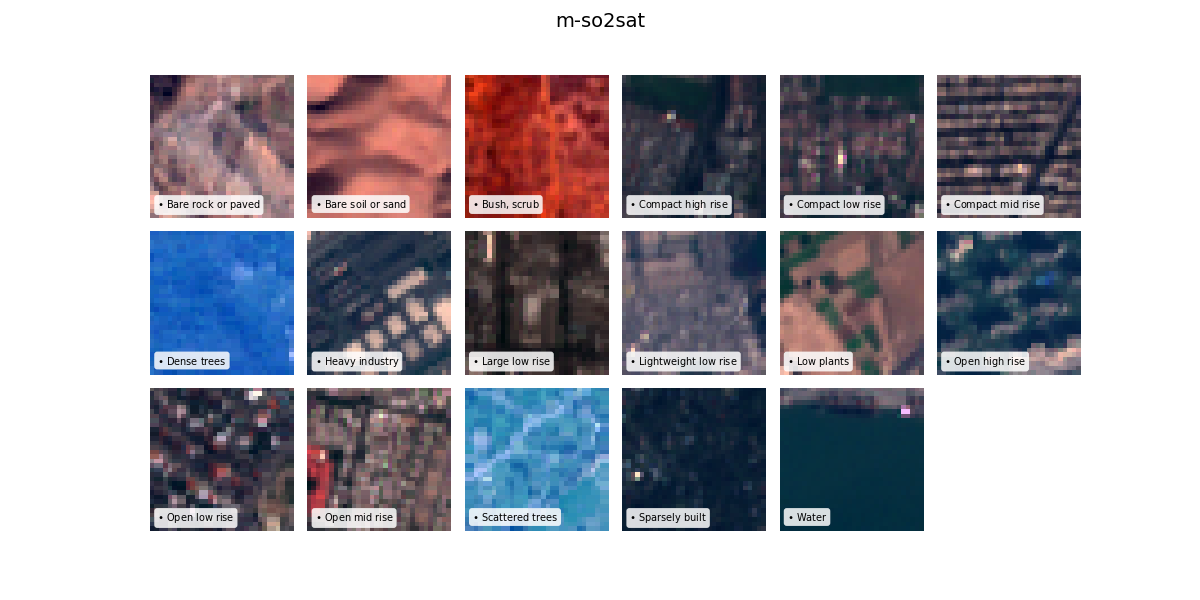
\includegraphics[width=\textwidth]{img/m-so2sat_image_grid.png}
    \caption{\normalsize Sample images from the 17 classes contained in the m-so2sat dataset from GEO-Bench.}
    \label{fig:so2satgrid}
\end{figure}


\subsection{m-bigearthnet}

The m-bigearthnet dataset is the multispectral, multilabel classification task derived from the BigEarthNet-MM project \cite{sumbul2021bigearthnet}. Unlike previous GEO-Bench datasets, which are binary or multiclass in nature, m-bigearthnet introduces a multilabel setting, where each image may belong to multiple land cover categories simultaneously as shown in Figure \ref{fig:bengrid}. This more realistically reflects complex, mixed-use landscapes such as forested urban scenes, agriculture mosaics with water courses, bare rock islands or mountainous shrublands.
The GEO-Bench variant of this dataset is restricted to Sentinel-2 multispectral imagery only and contains $22,000$ image patches and corresponding labels from a pool of 43 land cover classes, based on the CORINE Land Cover (CLC) Level-3 nomenclature from 2018 (slightly refined to improve label coherence). In GEO-Bench, the m-bigearthnet dataset has been reformatted into $120\times 120$ images with 12 multispectral bands, again split into training, validation, and test partitions consistent with other GEO-Bench tasks. The labels are provided in the form of binary label vectors representing one-hot encoded multilabel annotations per image. Each label vector includes between 1 and 12 active labels, with a mean of 5-6 labels per image. This requires a Vision Language model like CLIP to compute the labels prediction with different strategies, as the task increases in complexity in many ways: the labels may contain semantic overlap, e.g. "pasture" and "agricultural land", there are issues of label imbalance, with some captions occurring more often and other more rarely, not to mention noisy annotations, that occasionally don't reflect all the true content of an image due to the fact that they were generated in an automatic, therefore not perfect way. Despite these complexities, m-bigearthnet is an invaluable benchmark for evaluating real-world multi-concept classification in Remote Sensing. With its scale, diversity, and affinity to human-like capabilities, it completes the GEO-Bench collection providing an intriguing stress-testing for models that aim to scale beyond simple classification schemes.

\begin{figure}[h]
    \centering
    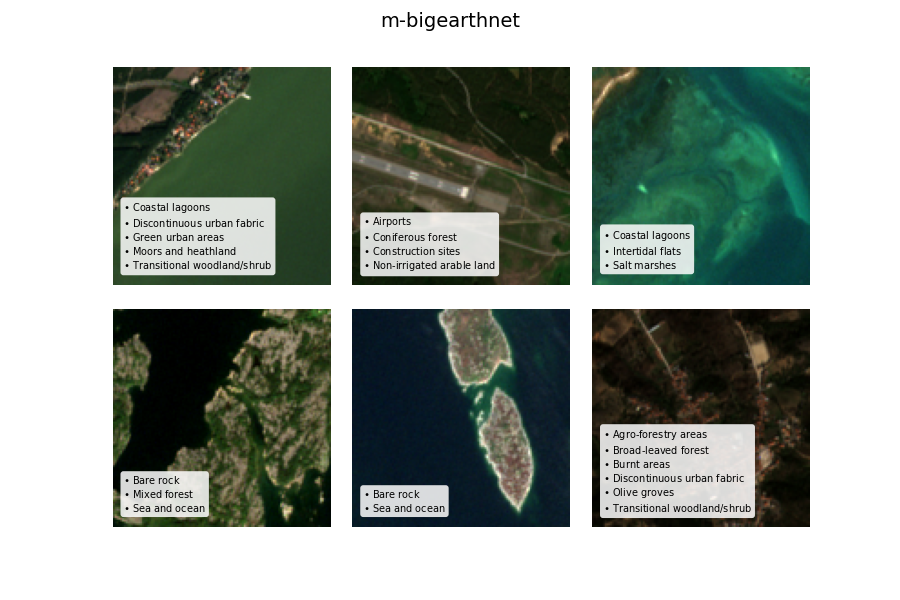
\includegraphics[width=\textwidth]{img/m-bigearthnet_image_grid.png}
    \caption{Sample multilabel images featured in the m-bigearthnet dataset from GEO-Bench.}
    \label{fig:bengrid}
\end{figure}


\chapter{Approach} % ------------------------------------------

\section{Multi Spectral Embedders}

(Explain the concept)

Add pseudocode for the structure + small scheme of the pipeline, possibly including the size of the embedder (thinner block for MSI1, thicker for MSI2)

Structure the MSI embedder section to describe:

Motivation: Why not retrain or finetune CLIP?

Architecture: MSI1, MSI2, MSI-T (number of layers, kernel sizes, ReLU/batchnorm?)

Integration: How embeddings are passed to CLIP (e.g., matching 3-channel format via projection).

Include a diagram showing the pipeline: MSI image → embedder → CLIP encoder → similarity with text embeddings.


\subsection{MSI-1 Embedder}

(add some pseudocode)

\begin{figure}[ht]
\centering %put "linenos" in below [] to have numbered lines
    \begin{minted}[fontsize=\footnotesize, breaklines]{python} 
    # image_encoder  - ResNet or Vision Transformer
    # text_encoder   - CBOW or Text Transformer
    # I[n, h, w, c]  - minibatch of aligned images
    # T[n, l]        - minibatch of aligned texts
    # W_i[d_i, d_e]  - learned proj of image to embed
    # W_t[d_t, d_e]  - learned proj of text to embed
    # t              - learned temperature parameter
    
    # extract feature representations of each modality
    I_f = image_encoder(I)  #[n, d_i]
    T_f = text_encoder(T)   #[n, d_t]
    
    # joint multimodal embedding [n, d_e]
    I_e = l2_normalize(np.dot(I_f, W_i), axis=1)
    T_e = l2_normalize(np.dot(T_f, W_t), axis=1)
    
    # scaled pairwise cosine similarities [n, n]
    logits = np.dot(I_e, T_e.T) * np.exp(t)
    
    # symmetric loss function
    labels = np.arange(n)
    loss_i = cross_entropy_loss(logits, labels, axis=0)
    loss_t = cross_entropy_loss(logits, labels, axis=1)
    loss   = (loss_i + loss_t)/2
    \end{minted}
\caption{Numpy-like pseudocode for the core of an implementation of CLIP.}
\label{fig:clipcode}
\end{figure}


\subsection{MSI-2 Embedder}
\subsection{MSI-T Embedder}
\subsection{MSI-T-4L Embedder}


\section{MSI + CLIP Model Structure}

(add a schematization of where the embedder is placed in the model)

\paragraph{Base model}

(how the model works for specific datasets, adapting to the number of available bands, training and testing for the specific case)

\paragraph{Transfer Learning model}

(how the embedder trained on a specific dataset (and how that dataset was chosen) 

\chapter{Experimental setup} % --------------------------------

Justify use of ViT-B/32 (mention comparability with literature).

Be clear about what is frozen (CLIP) and what is trained (embedder).

In the normalization section, explain why per-channel dataset-wide normalization is preferred (statistical stability across scenes).


This project focuses on some ground benchmarking work in the scope of \emph{image classification}. This task has been chosen for reasons like a lack of baseline results to compare CLIP-like models to different types of VLMs, but also between themselves. Given the versatility of these models and the possible application to several types of tasks, the literature disagrees/is not uniform in the tasks (and consequentially in the evaluation) of these models. For simplicity, and to make the results more significant in the context of existing literature, and to fill small research gaps that miss a comprehensive evaluation of these models, we choose here to focus on classification (also for the "universality" of this task, it's easy to understand, it's easy to compare models on it). Therefore, we adopt the classic classification evaluation metrics for the binary and multiclass tasks, while some more research has been carried out to evaluate the multilabel task as it needs to be treated a bit differently.

\section{Evaluation metrics}

\paragraph{Binary/Multiclass Classification}

\begin{itemize}
    \item \textbf{Accuracy}:
    \item \textbf{Precision}:
    \item \textbf{Recall}:
    \item \textbf{F1 Score}:
    \item \textbf{Confusion Matrix}
\end{itemize}

\paragraph{Multilabel Classification}

\begin{itemize}
    \item \textbf{Precision@k (P@k)}:
    \item \textbf{Recall@k (R@k)}:
    \item \textbf{Mean Average Precision (mAP)}:
    \item \textbf{Micro F1}:
    \item \textbf{Ranking Loss}:
\end{itemize}


\section{Baseline tests}

\paragraph{EuroSAT}

\begin{table}[h]
\centering
\footnotesize
\renewcommand{\arraystretch}{1.2}
    \begin{tabular}{llc}
    \specialrule{.1em}{.2em}{.2em}
    \textbf{Model} & \textbf{Backbone} & \textbf{EuroSAT} \\
    \specialrule{.06em}{.2em}{.2em}
    CLIP        & ViT-B/32 & 38.76\% \\ 
    RemoteCLIP  & ViT-B/32 & 37.34\% \\
    GeoRSCLIP   & ViT-B/32 & \textbf{53.54\%} \\
    SkyCLIP     & ViT-B/32 & 52.26\% \\
    \specialrule{.1em}{.2em}{.2em}
    \end{tabular}
\vspace{0.3cm}
\caption{\normalsize Comparison of zero-shot accuracies obtained by different models on the EuroSAT original dataset.}
\label{tab:eurobaselines}
\end{table}


\begin{figure}[h]
  \begin{subfigure}[t]{.5\textwidth}
    \centering
    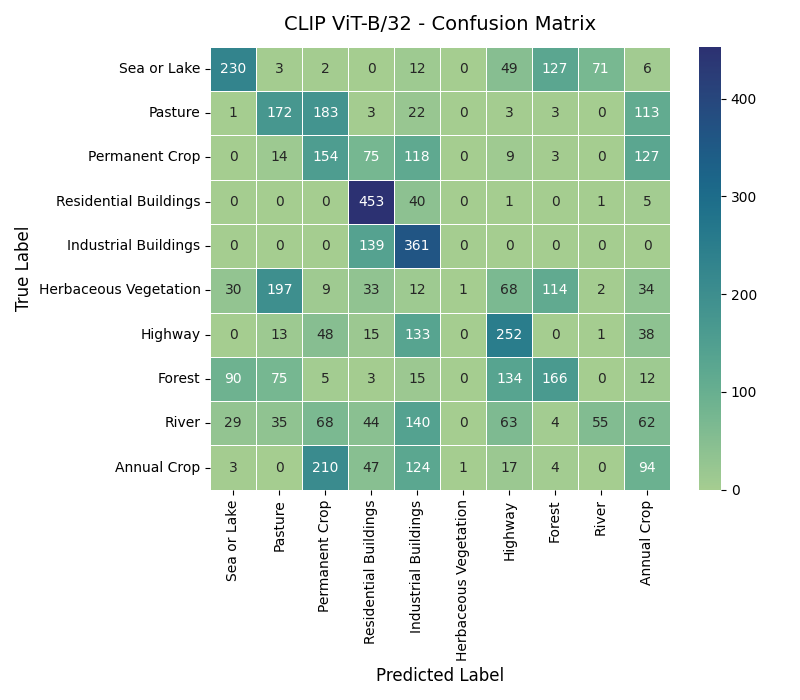
\includegraphics[width=\linewidth]{img/EuroSAT_CLIP_32_cm.png}
    %\caption{}
  \end{subfigure}
  \hfill
  \begin{subfigure}[t]{.5\textwidth}
    \centering
    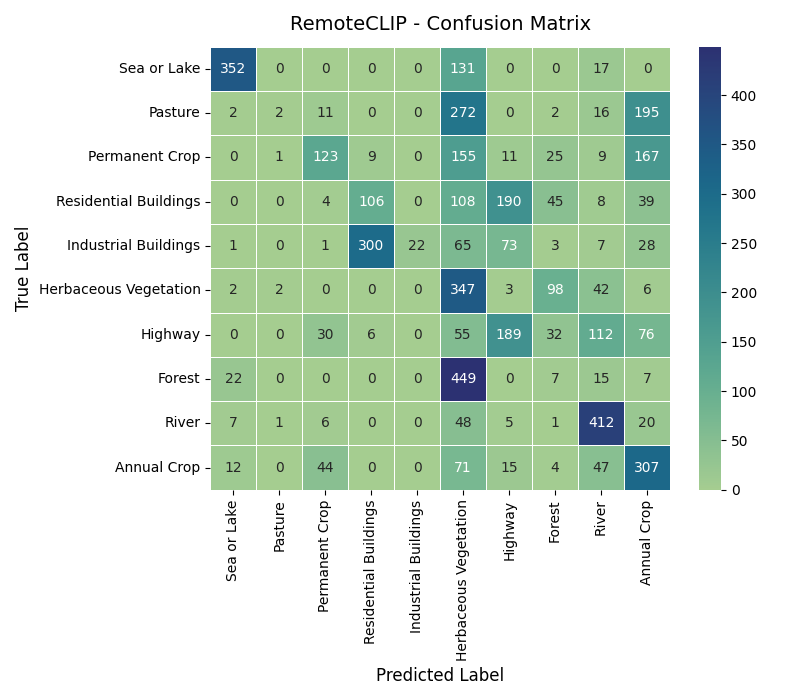
\includegraphics[width=\linewidth]{img/EuroSAT_RemoteCLIP_32_cm.png}
    %\caption{}
  \end{subfigure}

  \medskip

  \begin{subfigure}[t]{.5\textwidth}
    \centering
    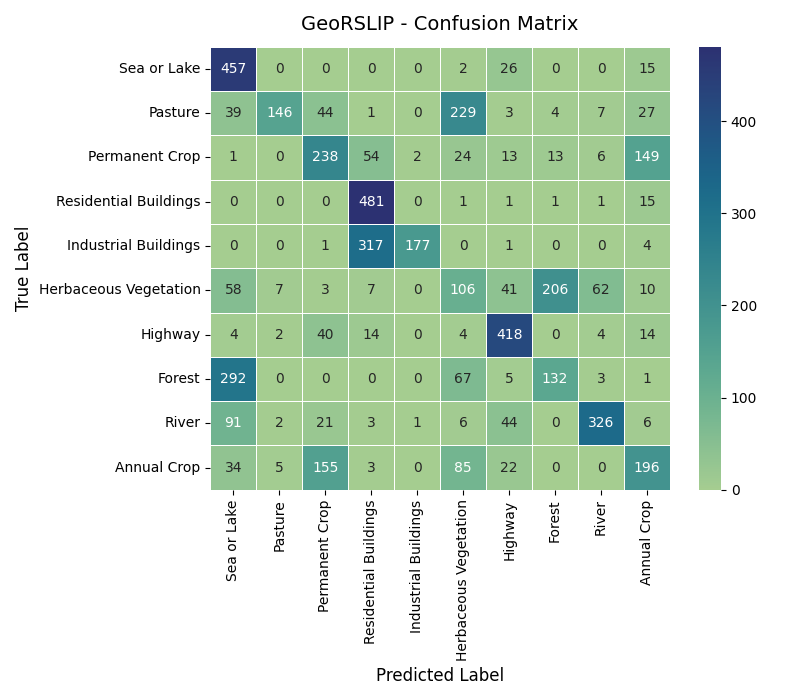
\includegraphics[width=\linewidth]{img/EuroSAT_GeoRSCLIP_32_cm.png}
    %\caption{}
  \end{subfigure}
  \hfill
  \begin{subfigure}[t]{.5\textwidth}
    \centering
    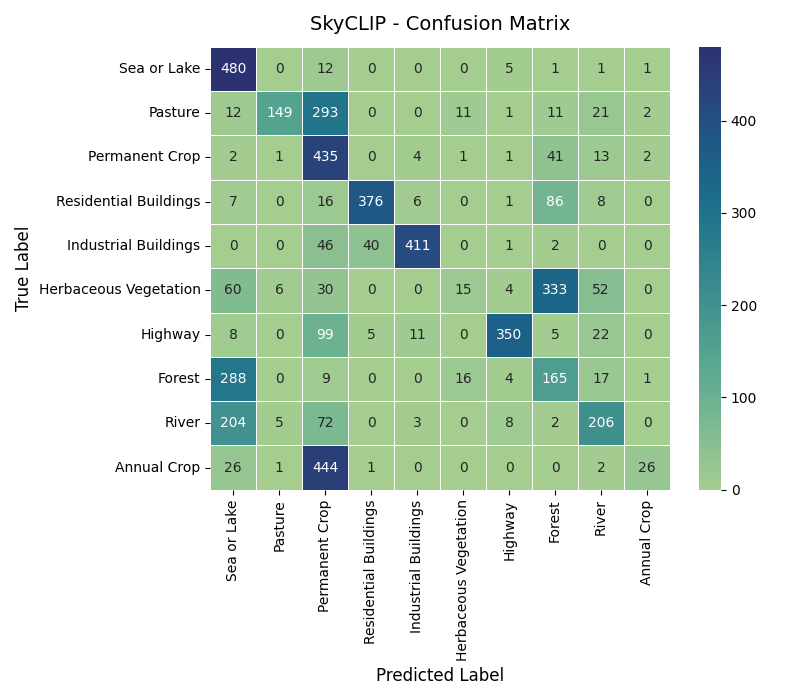
\includegraphics[width=\linewidth]{img/EuroSAT_SkyCLIP_32_cm.png}
    %\caption{}
  \end{subfigure}
  \caption{Confusion matrices of CLIP and other CLIP-like models finetuned on Remote Sensing datasets, evaluated on EuroSAT: while CLIP and RemoteCLIP's matrices appear somewhat fuzzy and struggle to recognize some classes at all, GeoRSCLIP and SkyCLIP's ones feature a more definite diagonal.}
\end{figure}



\paragraph{GEO-Bench}


\begin{table}[ht]
\centering
\footnotesize
\renewcommand{\arraystretch}{1.2}
    \begin{tabular}{llccccc}
    %\hline
    \specialrule{.1em}{.2em}{.2em}
    \textbf{Model} & \textbf{Backbone} & \textbf{m-brick-kiln} & \textbf{m-pv4ger} & \textbf{m-forestnet} & \textbf{m-eurosat} & \textbf{m-so2sat} \\
    %{} & {} & \textbf{acc} & \textbf{acc} & \textbf{acc} & \textbf{acc} & \textbf{acc} \\
    %\hline
    \specialrule{.06em}{.2em}{.2em}
    CLIP        & ViT-B/32 & \textbf{70.27\%} & 73.87\% & 7.65\% & 41.90\% & \textbf{16.63\%}\\ %\hdashline[2pt/5pt]
    RemoteCLIP  & ViT-B/32 & 66.97\% & 65.97\% & 8.25\% & 28.70\% & 12.78\% \\
    GeoRSCLIP   & ViT-B/32 & 68.67\% & 89.09\% & \textbf{14.20\%} & \textbf{51.30\%} & 15.82\% \\
    SkyCLIP     & ViT-B/32 & 59.36\% & \textbf{90.59\%} & 10.67\% & 49.30\% & 12.27\% \\
    %\hline
    \specialrule{.1em}{.2em}{.2em}
    \end{tabular}
\vspace{0.3cm}
\caption{\normalsize Comparison of zero-shot accuracies obtained by different models across GEO-Bench datasets.}
\label{tab:baselines}
\end{table}


\begin{table}[ht]
\centering
\footnotesize
\renewcommand{\arraystretch}{1.2}
    \begin{tabular}{llcccc|c}
    \toprule
    %\textbf{Model} & \textbf{Method} & \multicolumn{5}{c}{\textbf{m-bigearthnet}} \\
    \multirow{2}{*}{\textbf{Model}} & \multirow{2}{*}{\textbf{Backbone}} & \multicolumn{5}{c}{\textbf{m-bigearthnet}} \\
    \cmidrule(lr){3-7}
    & & \textbf{R@5} & \textbf{P@5} & \textbf{mAP} & \textbf{F1} & \textbf{rloss} \\
    \specialrule{.06em}{.2em}{.2em}
    CLIP        & ViT-B/32 & 31.70\% & 23.40\% & 32.32\% & 20.39\% & 28.71\% \\ 
    RemoteCLIP  & ViT-B/32 & 26.24\% & 19.82\% & 27.63\%  & 20.30\% & 30.89\%  \\
    GeoRSCLIP   & ViT-B/32 & \textbf{38.89\%} & \textbf{28.60\%} & \textbf{39.69\%} & 22.15\% & \textbf{23.19\%} \\
    SkyCLIP     & ViT-B/32 & 26.53\% & 19.30\% & 28.61\% & \textbf{22.39\%} & 30.98\%  \\
    \bottomrule
    \end{tabular}
\vspace{0.3cm}
\caption{\normalsize Comparison of zero-shot performance metrics obtained by different models on the m-bigearthnet dataset from GEO-Bench.}
\label{tab:baselines-multilab}
\end{table}


\section{Text prompts experiments}

* Focus on binary classification *

- Explain the problems with negation, cite paper \cite{quantmeyer2024and}

- Explain the idea behind the binary approach and the one behind the multi-prompt approach

(from CLIP's original paper, valid not only for text prompts experiment but also baseline tests)

Another issue we encountered is that it’s relatively rare in our pre-training dataset for the text paired with the image to be just a single word. Usually the text is a full sentence describing the image in some way. To help bridge this distribution gap, we found that using the prompt template “A photo of a {label}.” to be a good default that helps specify the text is about the content of the image. This often improves performance over the baseline of using only the label text.

Finally, we found that on satellite image classification datasets it helped to specify that the images were of this form and we use variants of “a satellite photo of a {label}.”.


\paragraph{m-brick-kiln}

TODO: List the prompts and the corresponding mapping to positive/negative classes


\begin{table}[ht]
\centering
\footnotesize
\renewcommand{\arraystretch}{1.2}
    \begin{tabular}{lc|cccc}
    \toprule
    %\textbf{Model} & \textbf{original} & \textbf{Prompt 1} & \textbf{Prompt 2} & \textbf{Prompt 3} & \textbf{Multi-Prompt} \\
    \multirow{2}{*}{\textbf{Model}} & \multicolumn{4}{c}{\textbf{Binary Prompts}} &  \multirow{2}{*}{\textbf{Multi-Prompt}}\\
    \cmidrule(lr){2-5}
    & \textbf{Original} & \textbf{Type 1} & \textbf{Type 2} & \textbf{Type 3} \\
    \midrule
    CLIP & 70.27\% & 76.58\% & 80.38\% & 79.78\% & \textbf{83.58\%} \\
    RemoteCLIP & 66.97\% & 66.27\% & 66.77\% & \textbf{67.47\%} & 66.57\% \\
    GeoRSCLIP & 68.67\% & 71.87\% & 70.57\% & \textbf{73.37\%} & 68.17\%\\
    SkyCLIP & 59.36\% & 69.07\% & \textbf{69.27\%} & 69.17\% & 67.57\% \\ 
    \bottomrule
    \end{tabular}
\vspace{0.3cm}
\caption{\normalsize CLIP performance on m-brick-kiln with different text prompts.}
\label{tab:prompts1}
\end{table}


\paragraph{m-pv4ger}

TODO: List the prompts and the corresponding mapping to positive/negative classes


\begin{table}[ht]
\centering
\footnotesize
\renewcommand{\arraystretch}{1.2} % increase row spacing
    \begin{tabular}{lc|cccc}
    \toprule
    %\textbf{Model} & \textbf{original} & \textbf{Prompt 1} & \textbf{Prompt 2} & \textbf{Prompt 3} & \textbf{Multi-Prompt} \\
    \multirow{2}{*}{\textbf{Model}} & \multicolumn{4}{c}{\textbf{Binary Prompts}} &  \multirow{2}{*}{\textbf{Multi-Prompt}}\\
    \cmidrule(lr){2-5}
    & \textbf{Original} & \textbf{Type 1} & \textbf{Type 2} & \textbf{Type 3} \\
    \midrule
    CLIP & 73.87\% & 71.57\% & 79.28\% & 76.78\% & \textbf{82.88\%} \\
    RemoteCLIP & 65.97\% & 45.85\% & 48.15\% & 32.03\% & \textbf{74.47\%} \\
    GeoRSCLIP & 89.09\% & \textbf{94.19\%} & 93.29\% & 93.89\% & 92.09\% \\
    SkyCLIP & 90.59\% & 91.99\% & 90.79\% & 91.59\% & \textbf{92.09\%} \\
    \bottomrule
    \end{tabular}
\vspace{0.3cm}
\caption{\normalsize CLIP performance on m-pv4ger with different text prompts.}
\label{tab:prompts2}
\end{table}


\section{Image normalization experiments}

\begin{figure}[h]
    \centering
    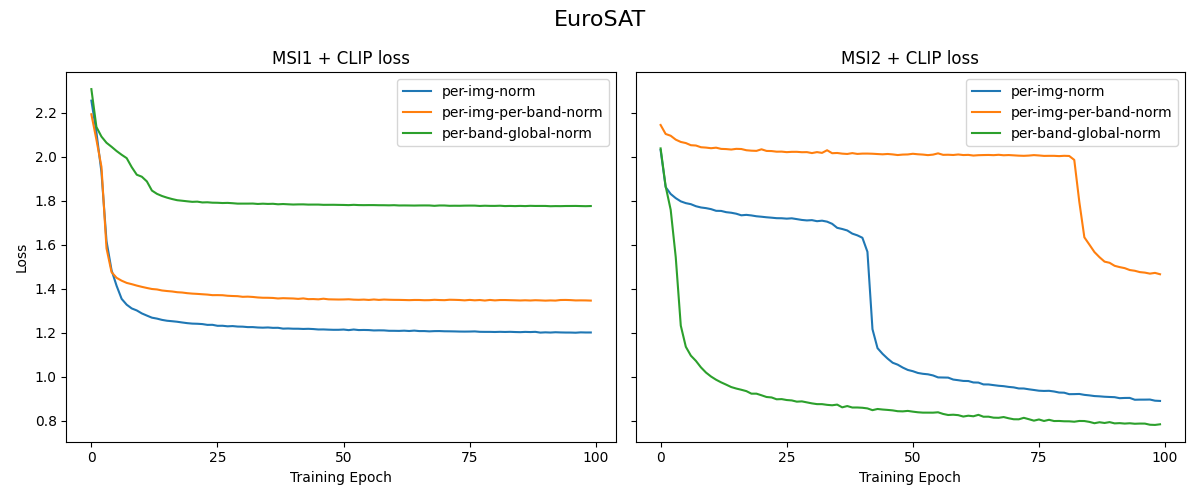
\includegraphics[width=\textwidth]{img/EuroSAT_norm_losses_plot.png}
    \caption{The effect of different normalization functions on the convergence of the training loss for the two different models.}
    \label{fig:normlosses}
\end{figure}

- comments of what normalization works best for the different models, how we calculated them, lin min max, cite \cite{unknown}, etc - 

Mention that to keep integrity and consistency with the dataset we adopt norm3 for all the following experiments and training.


\chapter{Results} % -------------------------------------------


Use a consistent format for results: for each dataset, report:

Zero-shot baseline

MSI1 + CLIP

MSI2 + CLIP

MSI-T + CLIP

RemoteCLIP / GeoRSCLIP / SkyCLIP (for context)

For transfer learning, consider a matrix format showing cross-dataset performance (e.g., trained on X → tested on Y).

Discuss why transfer learning failed in some cases (domain shift, band mismatch, overfitting to captions).


\section{Finetuning results}


\paragraph{EuroSAT}


\begin{table}[h]
\centering
\footnotesize
\renewcommand{\arraystretch}{1.2}
    \begin{tabular}{ccc}
    \specialrule{.1em}{.2em}{.2em}
    \textbf{Model} & \textbf{Method} & \textbf{EuroSAT} \\
    \specialrule{.06em}{.2em}{.2em}
    CLIP        & zero-shot & 38.76\% \\ 
    | &  | & | \\
    MSI1+CLIP & MSI1 training  & 37.29\% \\
    {} & $\pm\Delta$ & \textcolor{red}{-1.47\%} \\
    MSI2+CLIP & MSI2 training & \textbf{75.44\%} \\
    {} & $\pm\Delta$ & \textcolor{customgreen}{+36.68\%} \\
    \specialrule{.1em}{.2em}{.2em}
    \end{tabular}
\vspace{0.3cm}
\caption{\normalsize Comparison of accuracies obtained after training different embedders on the EuroSAT original dataset: the first embedder almost matches the zero shot performance, while the second nearly doubles it.}
\label{tab:eurosatmsi}
\end{table}



\paragraph{GEO-Bench}


\begin{table}[ht]
\centering
\footnotesize
\renewcommand{\arraystretch}{1.3} 
    \begin{tabular}{ccccccc}
    %\hline
    \specialrule{.1em}{.2em}{.2em}
    \textbf{Model} & \textbf{Method} & \textbf{m-brick-kiln} & \textbf{m-pv4ger} & \textbf{m-forestnet} & \textbf{m-eurosat} & \textbf{m-so2sat} \\
    %\hline
    \specialrule{.06em}{.2em}{.2em}
    CLIP      & zero-shot & 70.27\% & 73.87\% & 7.65\% & 41.90\% & \underline{16.63\%} \\
    | &  | & | & | & | &| & | \\
    MSI1+CLIP & MSI1 training & \underline{86.38\%} & \underline{92.19\%} & \textbf{10.67\%} & 44.40\% & 15.82\% \\
    {} & $\pm\Delta$ & \textcolor{customgreen}{+16.11\%} & \textcolor{customgreen}{+18.32\%} & \textcolor{customgreen}{+3.02\%} & \textcolor{customgreen}{+2.50\%} & \textcolor{red}{-0.81\%} \\
    MSI2+CLIP & MSI2 training & \textbf{90.19\%} & \textbf{92.89\%} & \underline{9.86\%} & \textbf{67.50\%} & \textbf{18.45\%} \\
    {} & $\pm\Delta$ & \textcolor{customgreen}{+19.92\%} & \textcolor{customgreen}{+19.02} & \textcolor{customgreen}{+2.21\%} & \textcolor{customgreen}{+25.60\%} & \textcolor{customgreen}{+1.82\%} \\
    \specialrule{.1em}{.2em}{.2em}
    \end{tabular}
\vspace{0.3cm}
\caption{\normalsize Comparison of models with respect to the original CLIP, after training the embedders: the score in bold refers to the best model and the underlined one to the second best.}
\label{tab:geobenchmsi}
\end{table}



\section{Transfer Learning results}

\begin{table}[ht]
\centering
\footnotesize
\renewcommand{\arraystretch}{1.3} 
    \begin{tabular}{ccccccc}
    %\hline
    \specialrule{.1em}{.2em}{.2em}
    \textbf{Model} & \textbf{Method} & \textbf{m-brick-kiln} & \textbf{m-pv4ger} & \textbf{m-forestnet} & \textbf{m-eurosat} & \textbf{m-so2sat} \\
    %\hline
    \specialrule{.06em}{.2em}{.2em}
    CLIP      & zero-shot & \textbf{70.27\%} & \underline{73.87\%} & 7.65\% & 41.90\% & \underline{16.63\%} \\
    | &  | & | & | & | &| & | \\
    MSI-T-s & zero shot & 56.35\% & 71.97\% & 8.76\% & 16.79\% & \textbf{20.08\%} \\
    (m-so2sat train) & $\pm\Delta$ & \textcolor{red}{-13.92\%} & \textcolor{red}{-1.90\%} & \textcolor{customgreen}{+1.11\%} & \textcolor{red}{-25.11\%} & \textcolor{customgreen}{+3.45\%} \\
    %\specialrule{.01em}{.2em}{.2em}
    MSI-T-E & zero shot & 62.46\% & 53.25\% & \underline{10.27\%} & \underline{46.79\%} & 9.43\% \\
    (EuroSAT train) & $\pm\Delta$ & \textcolor{red}{-7.81\%} & \textcolor{red}{-20.62\%} & \textcolor{customgreen}{+2.62\%} & \textcolor{customgreen}{+4.89\%} & \textcolor{red}{-7.20\%} \\
    %\specialrule{.01em}{.2em}{.2em}
     MSI-T-E-4L & zero shot & \underline{69.36\%} & \textbf{86.68\%} & \textbf{11.48\%} & \textbf{53.60\%} &  5.88\% \\
    (EuroSAT train) & $\pm\Delta$ & \textcolor{red}{-0.91\%} & \textcolor{customgreen}{+12.81\%} & \textcolor{customgreen}{+3.83\%} & \textcolor{customgreen}{+11.70\%} & \textcolor{red}{-10.75\%} \\
    %\hline
    \specialrule{.1em}{.2em}{.2em}
    \end{tabular}
\vspace{0.3cm}
\caption{\normalsize Comparison of models with respect to the original CLIP: the accuracy in bold refers to the best performing model, the underlined one to the second best.}
\label{tab:geobenchtransfer}
\end{table}




% Loss plots
\begin{figure}[h]
    \centering
    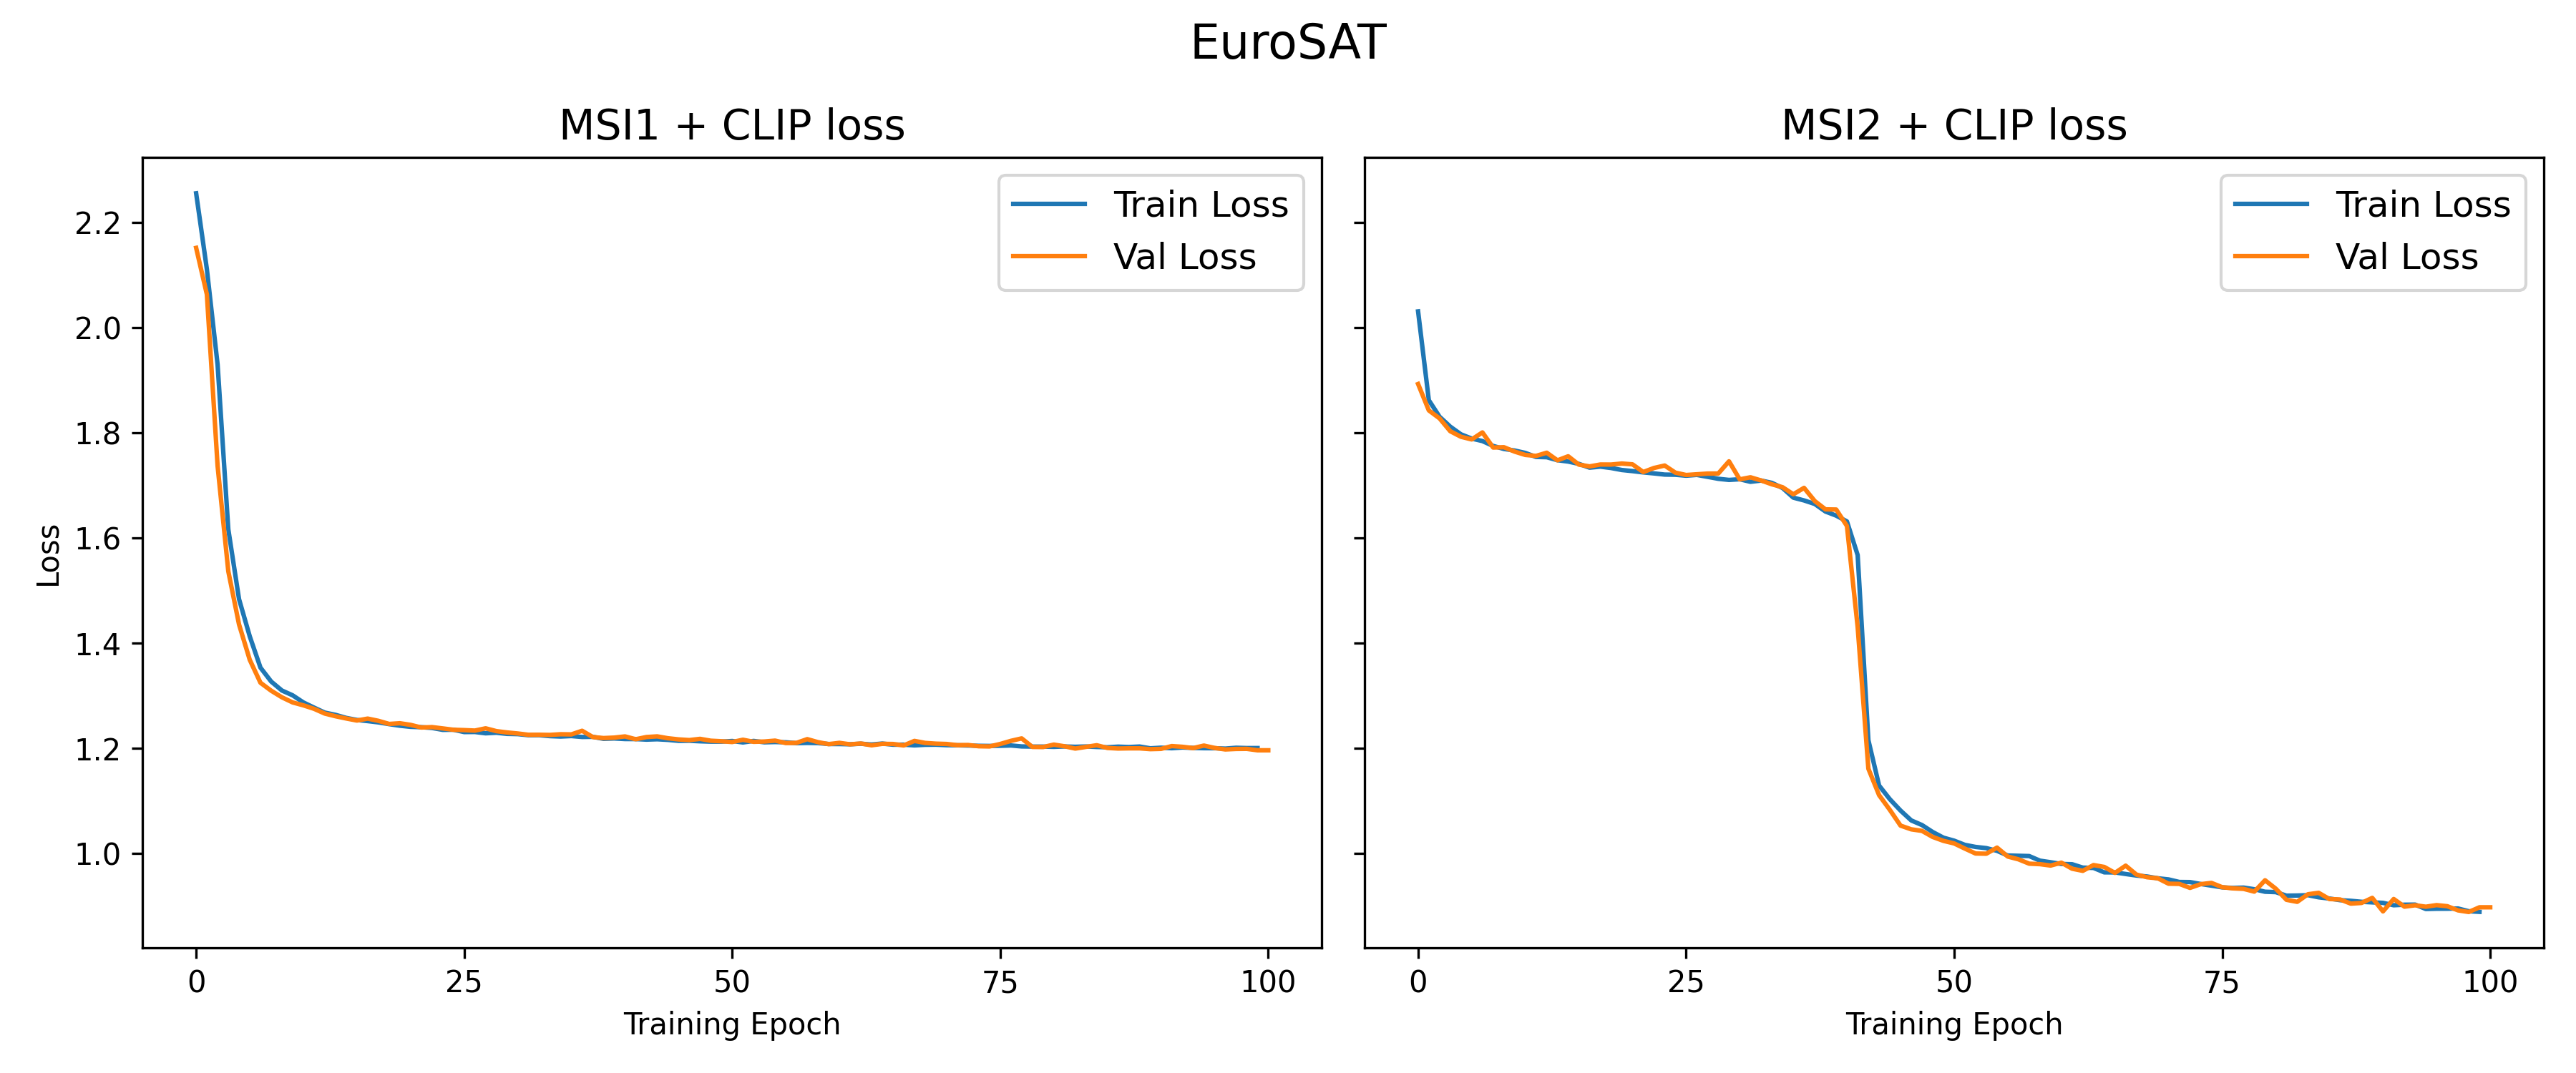
\includegraphics[width=\textwidth]{img/EuroSAT_loss_plot.png}
    \caption{Training and validation loss of the two embedders on the original EuroSAT dataset.}
    \label{fig:eurosatloss}
\end{figure}


\begin{figure}[h]
    \centering
    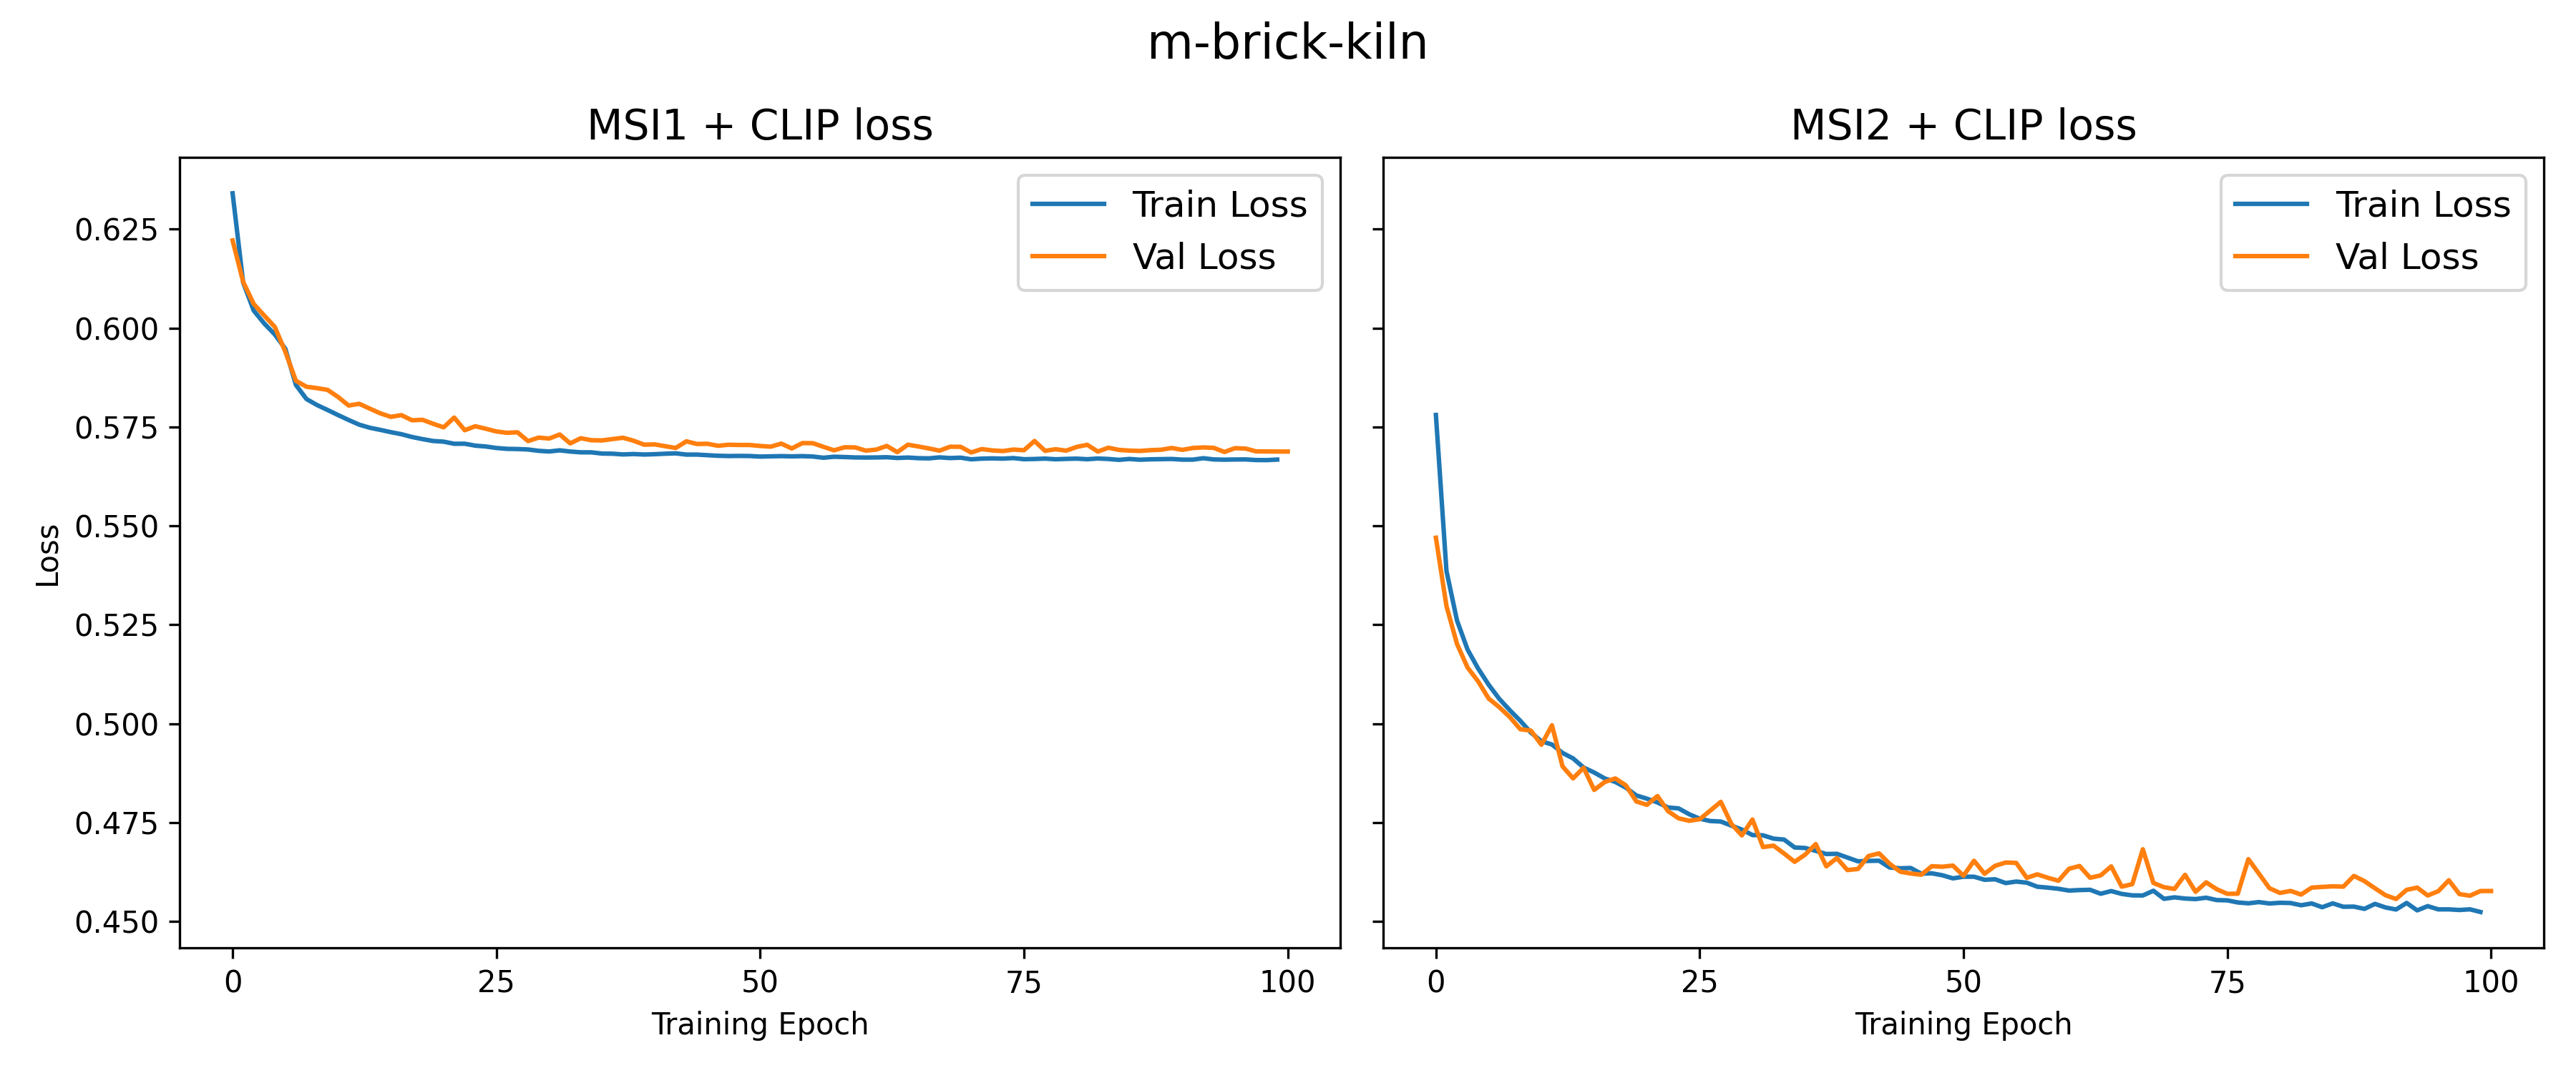
\includegraphics[width=\textwidth]{img/m-brick-kiln_loss_plot.png}
    \caption{Training and validation loss of the two embedders on the m-brick-kiln dataset from GEO-Bench.}
    \label{fig:brickloss}
\end{figure}

\begin{figure}[h]
    \centering
    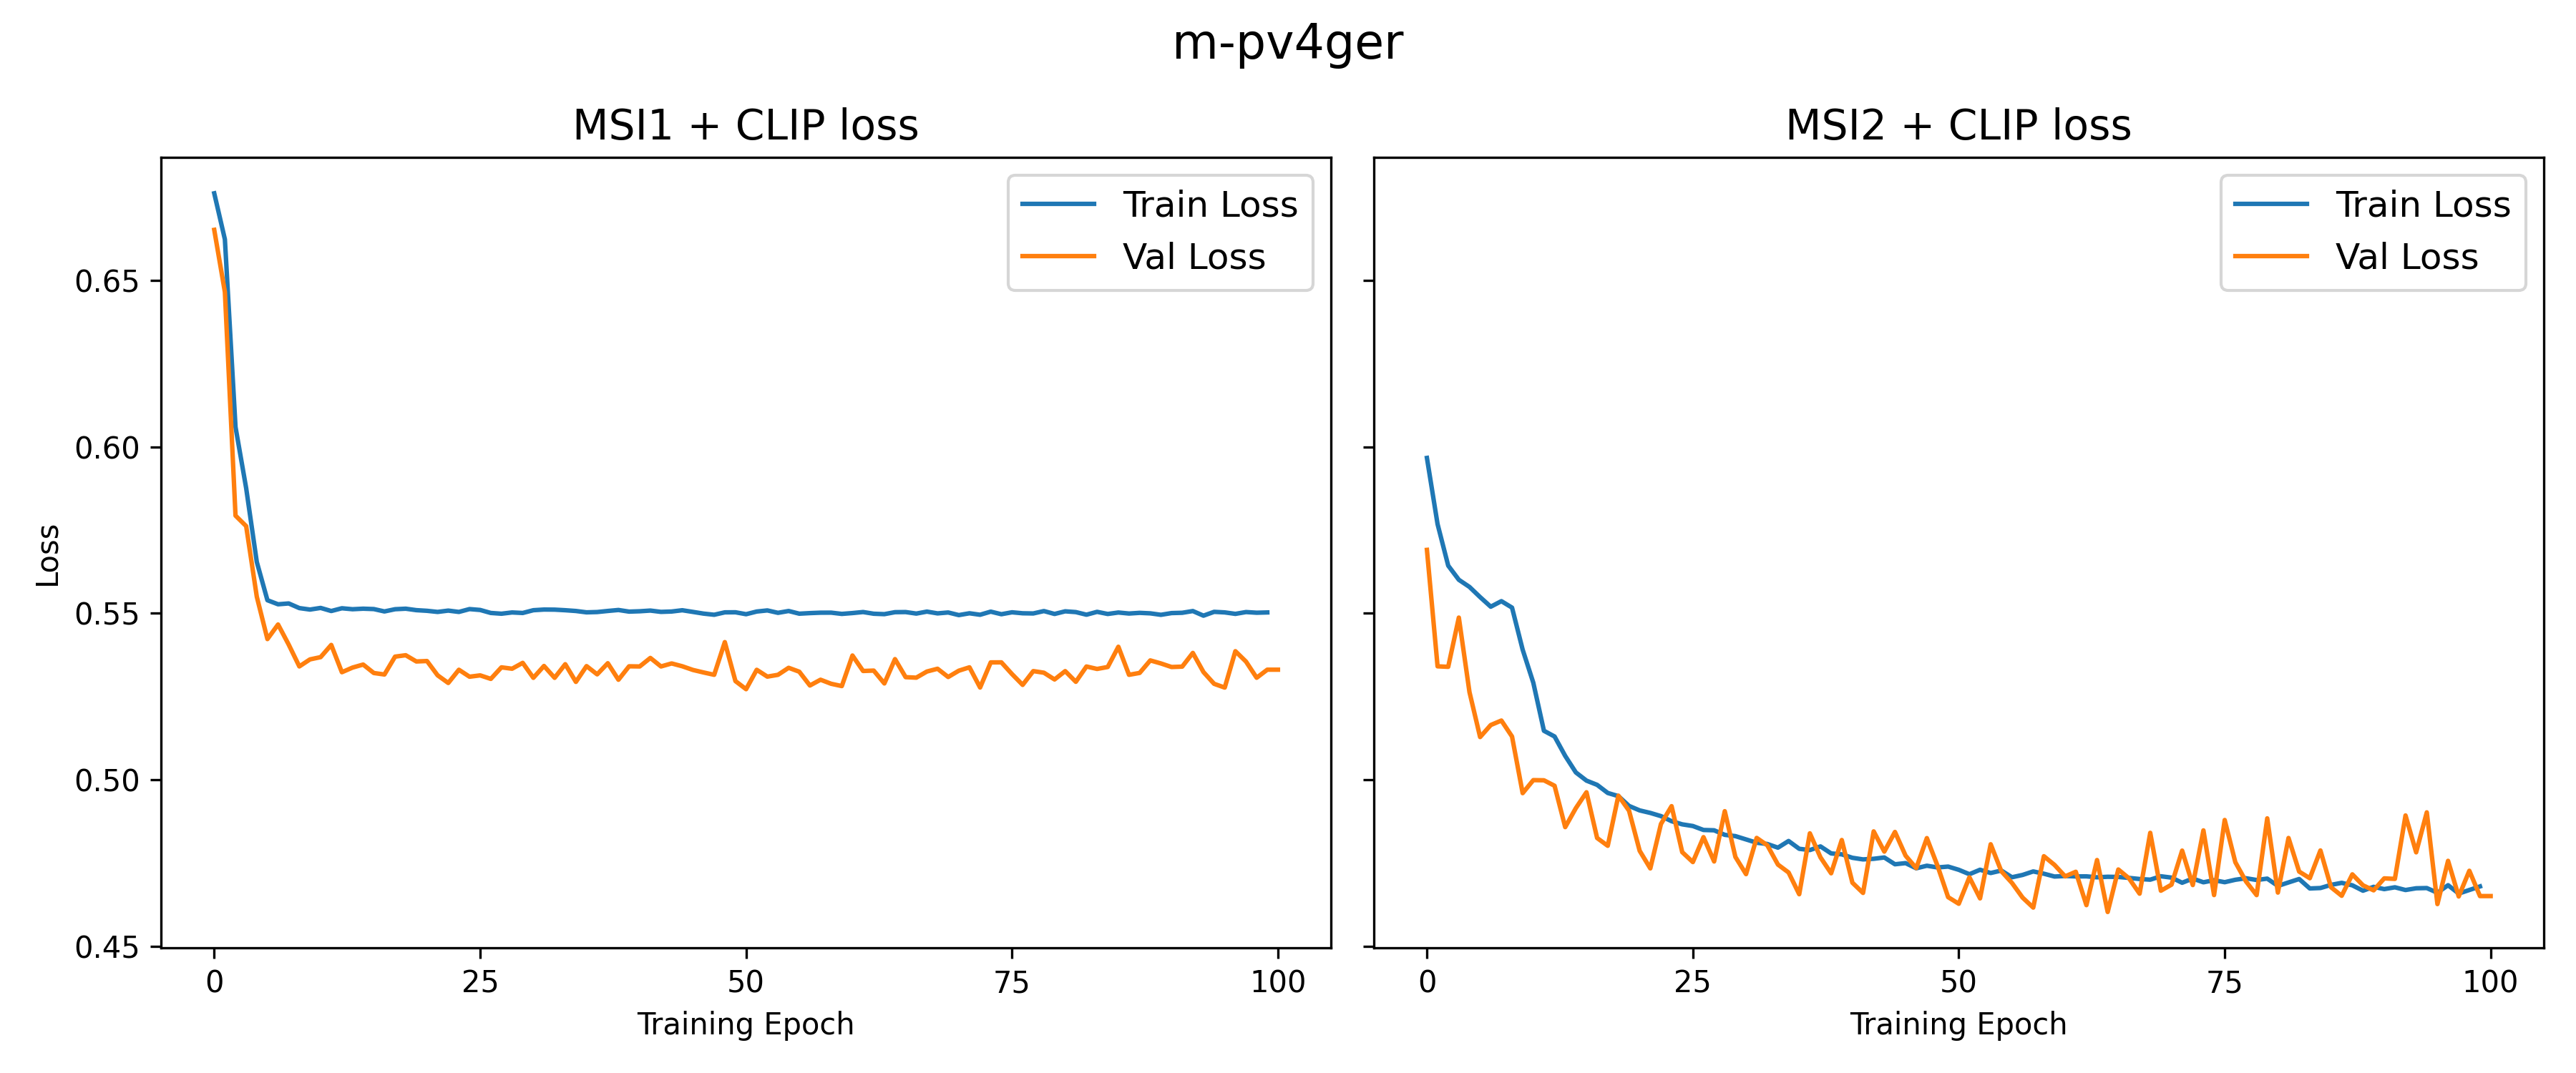
\includegraphics[width=\textwidth]{img/m-pv4ger_loss_plot.png}
    \caption{Training and validation loss of the two embedders on the m-pv4ger dataset from GEO-Bench.}
    \label{fig:solarloss}
\end{figure}

\begin{figure}[h]
    \centering
    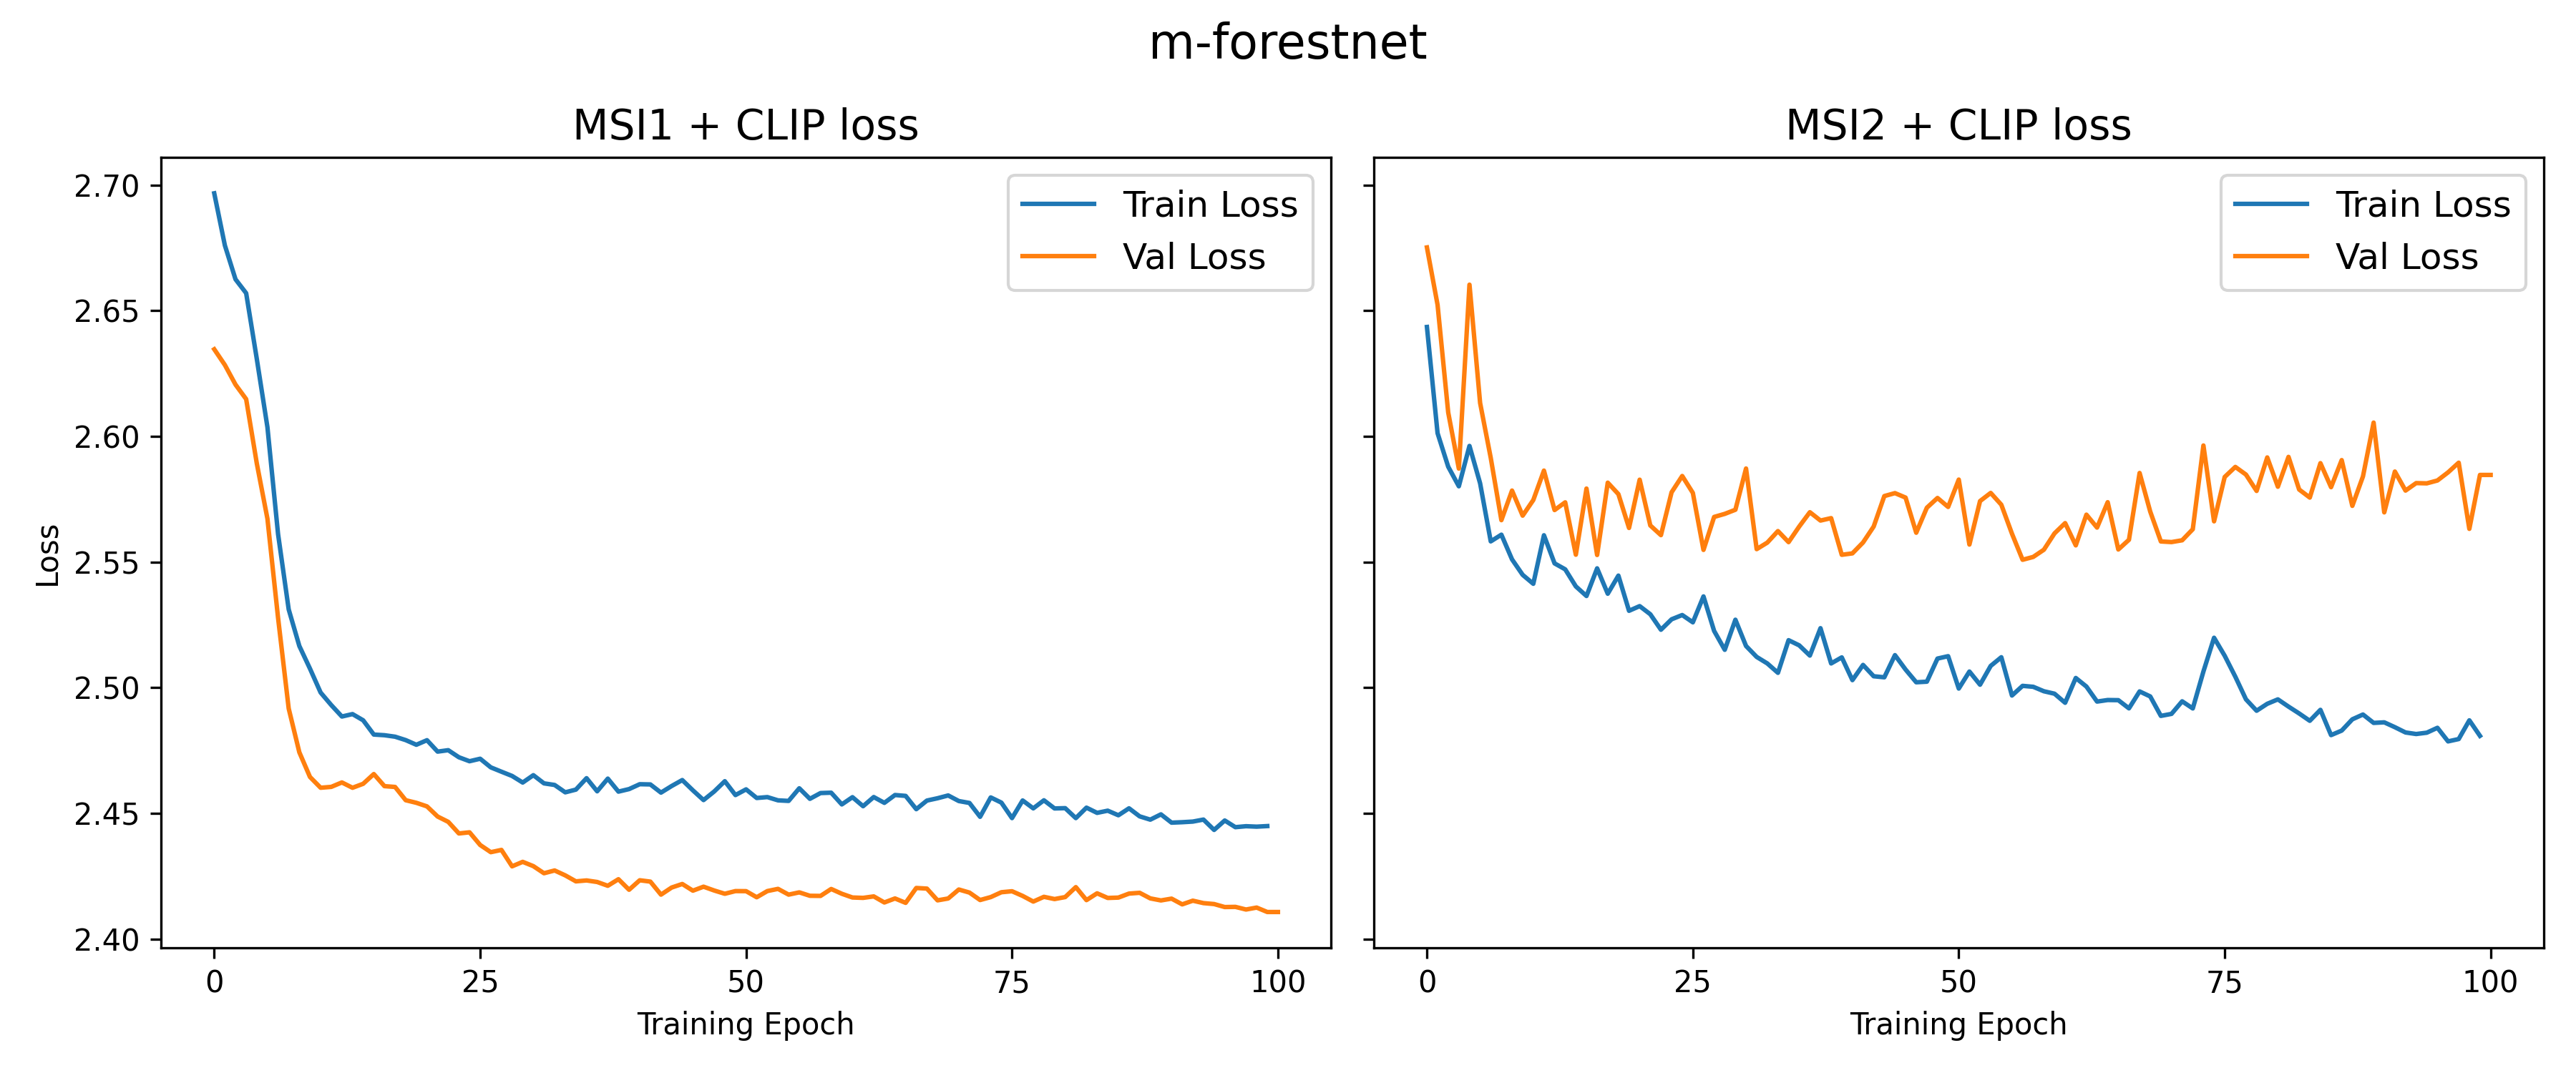
\includegraphics[width=\textwidth]{img/m-forestnet_loss_plot.png}
    \caption{Training and validation loss of the two embedders on the m-forestnet dataset from GEO-Bench.}
    \label{fig:foresloss}
\end{figure}

\begin{figure}[h]
    \centering
    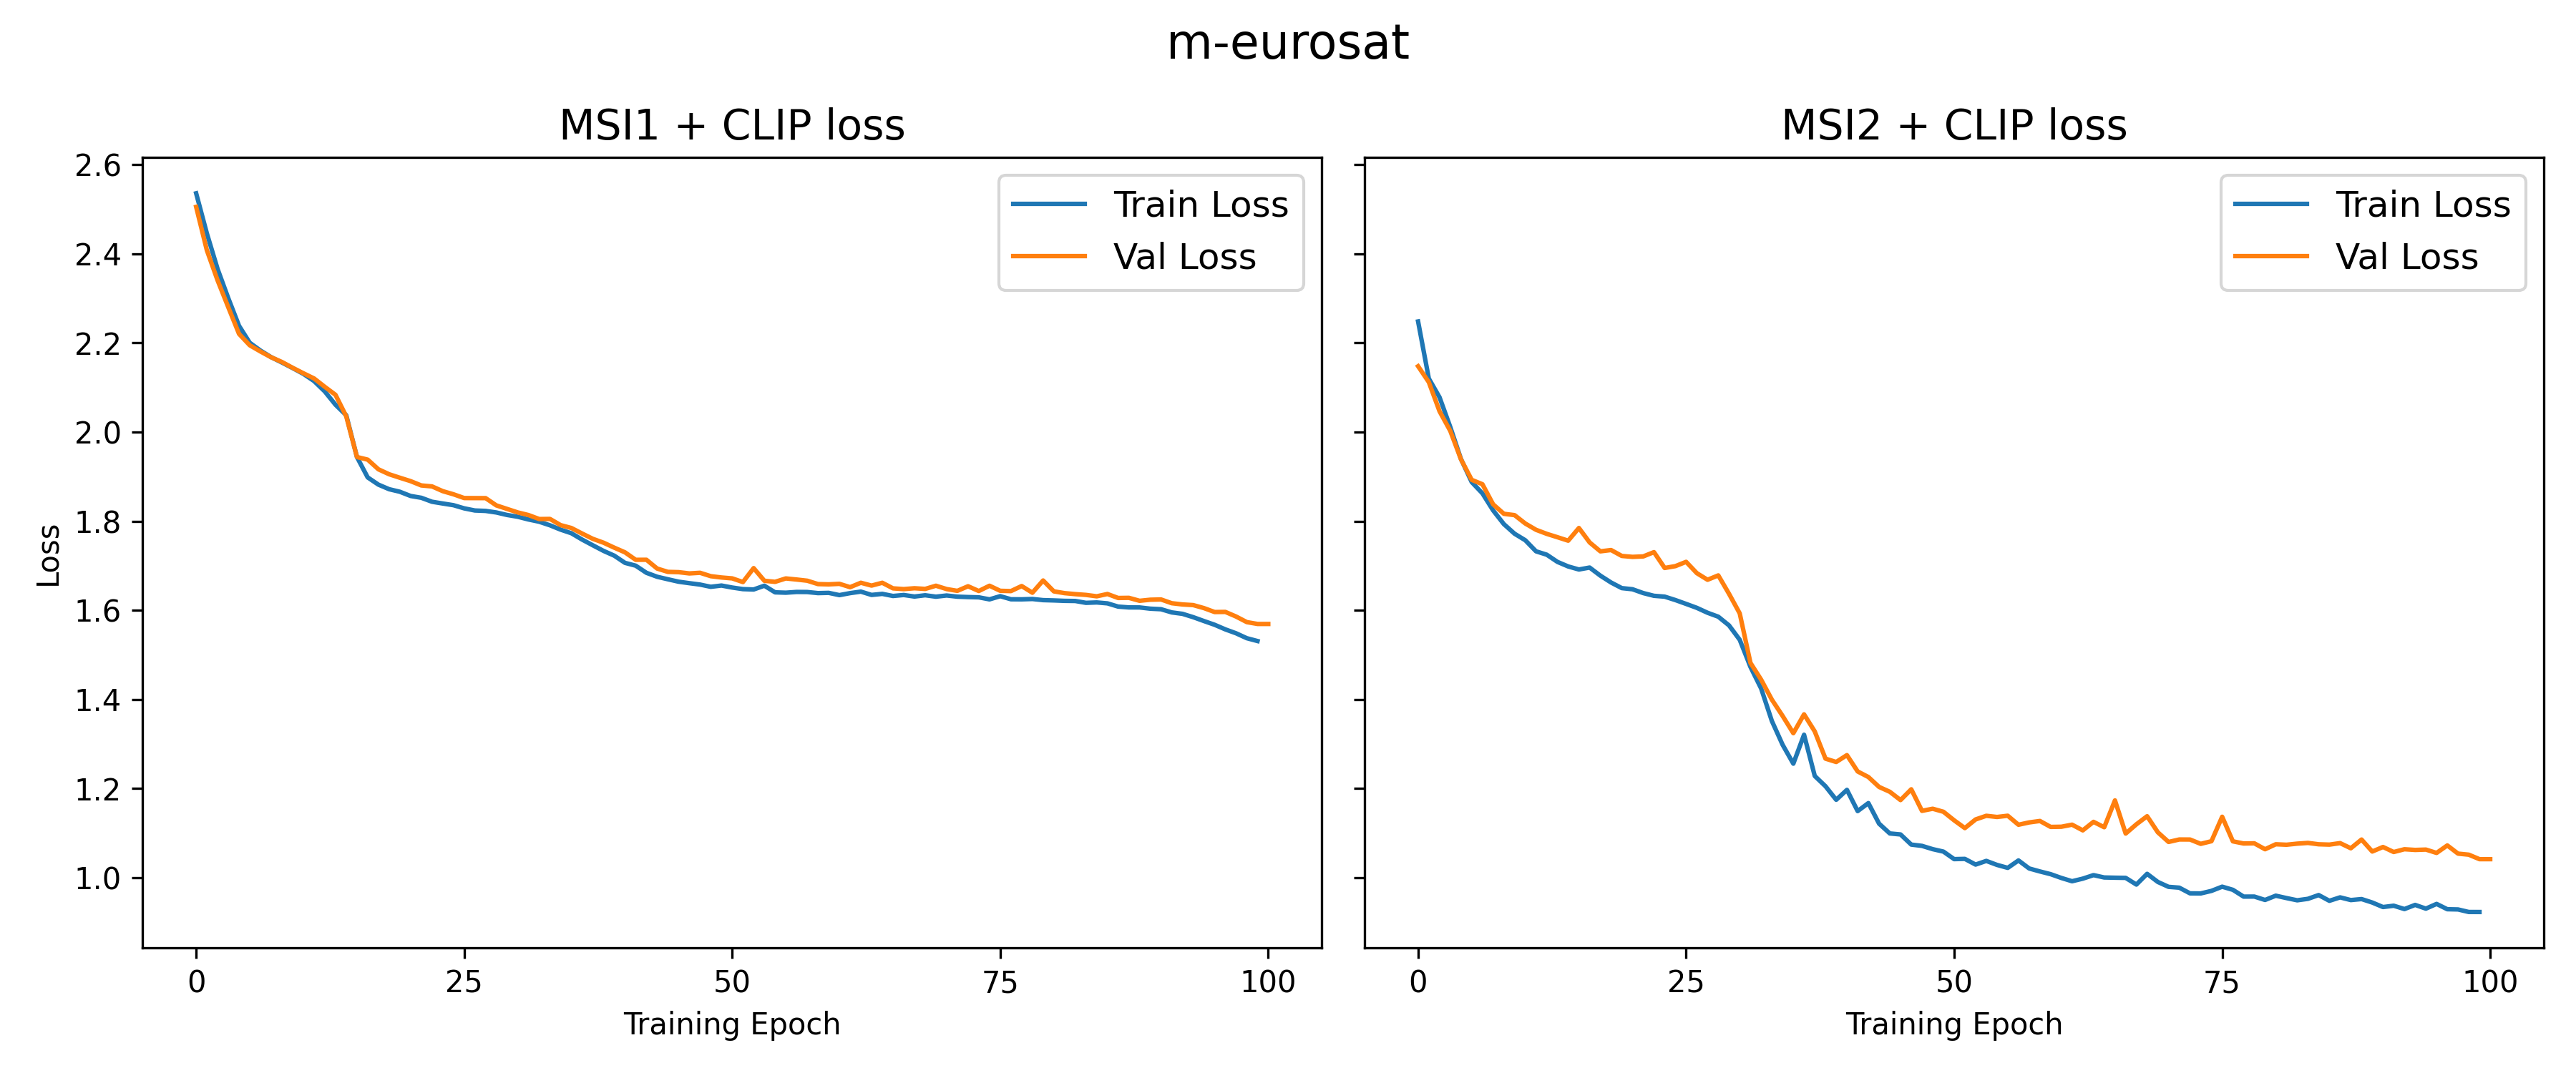
\includegraphics[width=\textwidth]{img/m-eurosat_loss_plot.png}
    \caption{Training and validation loss of the two embedders on the m-eurosat dataset from GEO-Bench.}
    \label{fig:meurosatloss}
\end{figure}

\begin{figure}[h]
    \centering
    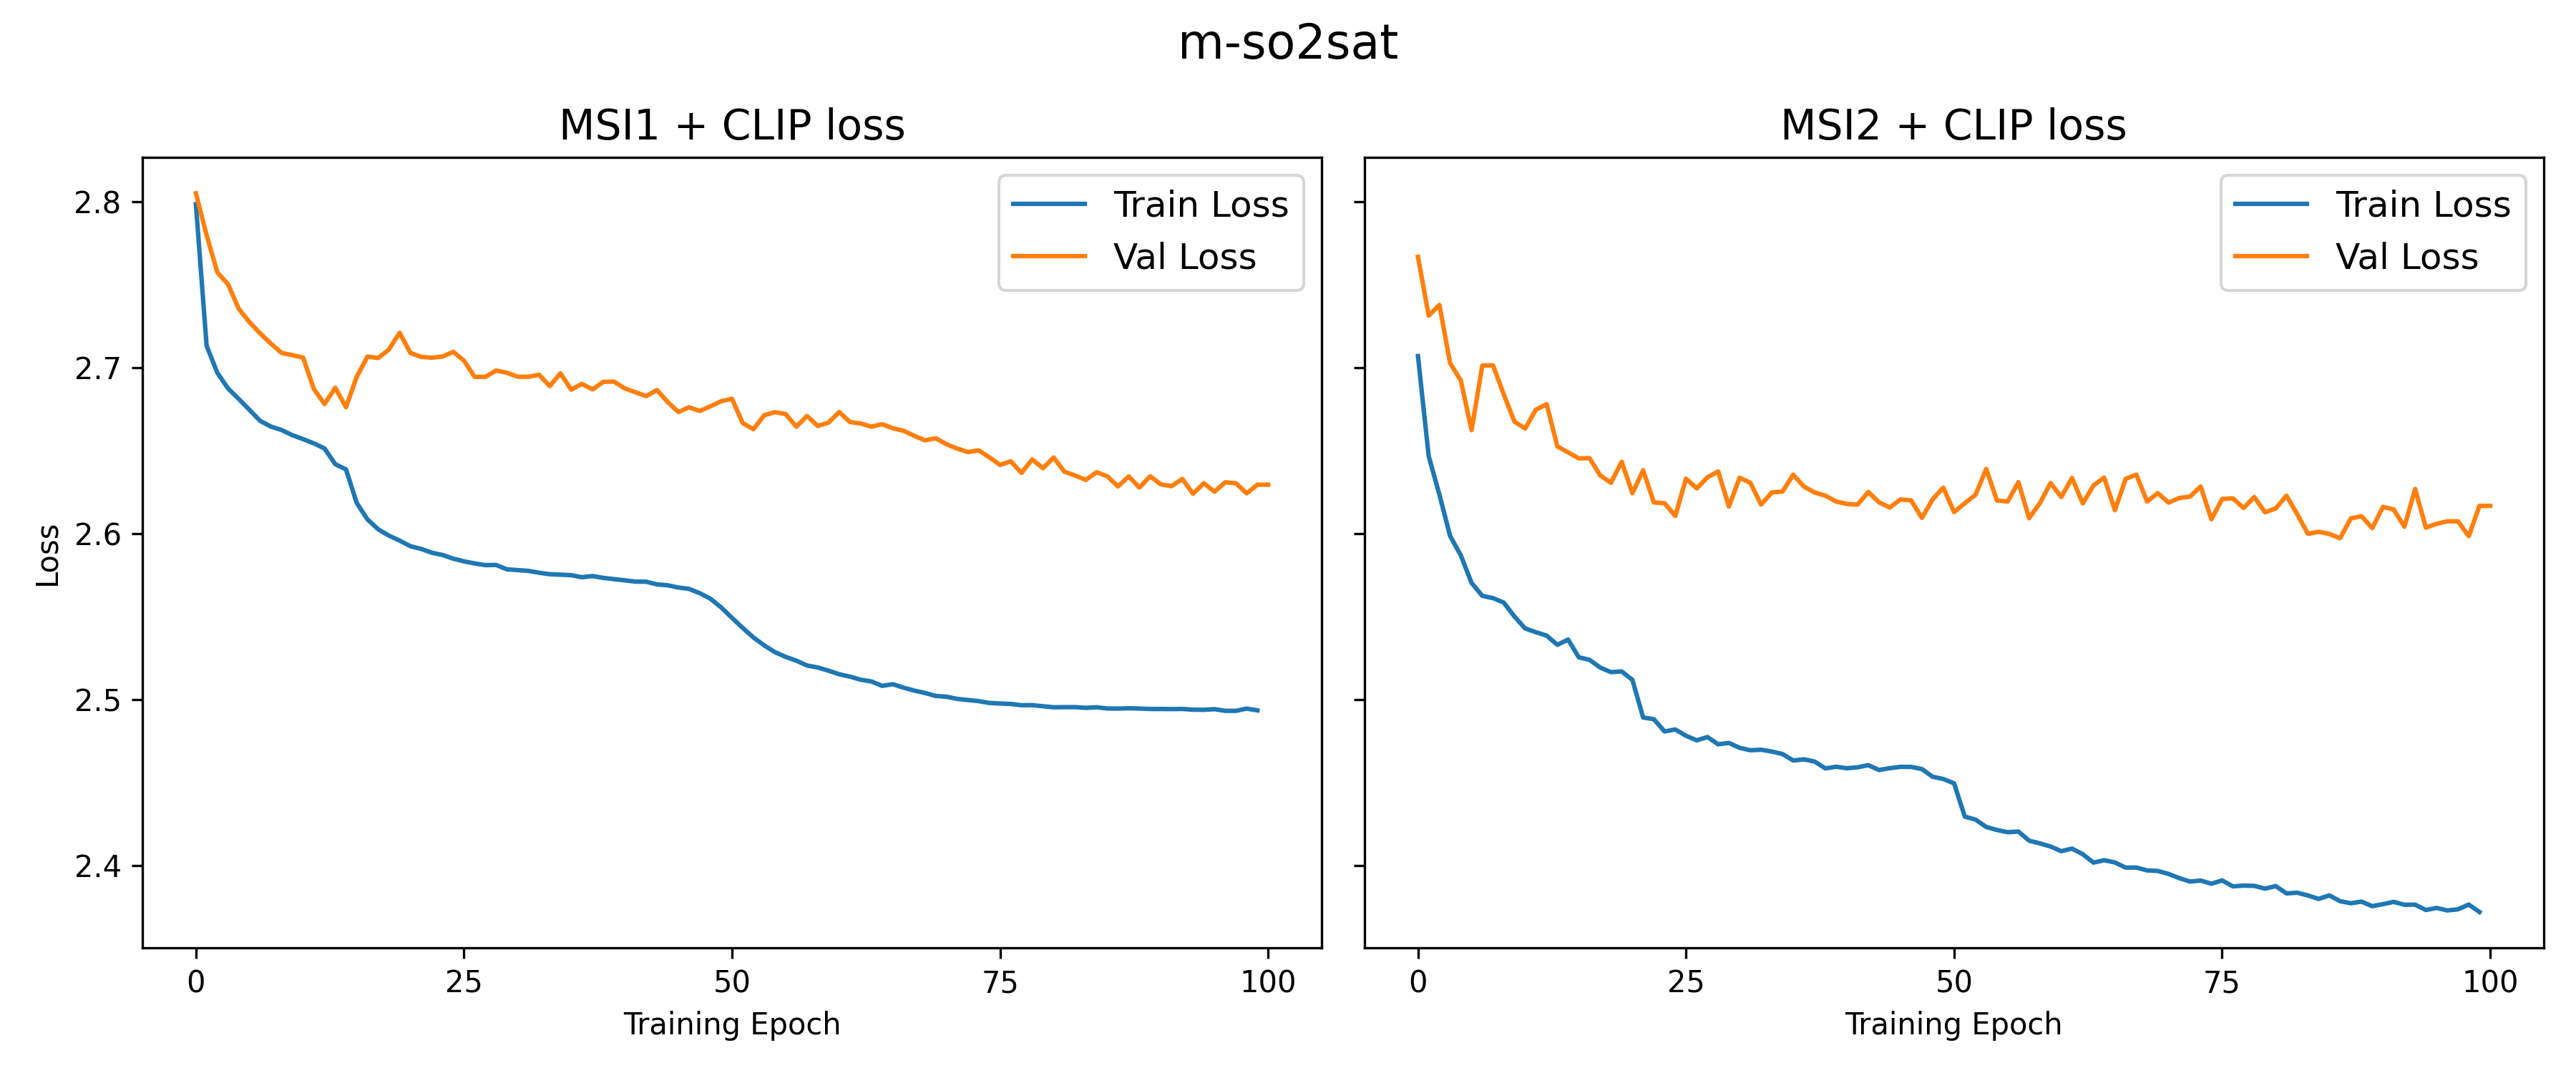
\includegraphics[width=\textwidth]{img/m-so2sat_loss_plot.png}
    \caption{Training and validation loss of the two embedders on the m-so2sat dataset from GEO-Bench.}
    \label{fig:so2satloss}
\end{figure}

\begin{figure}[h]
    \centering
    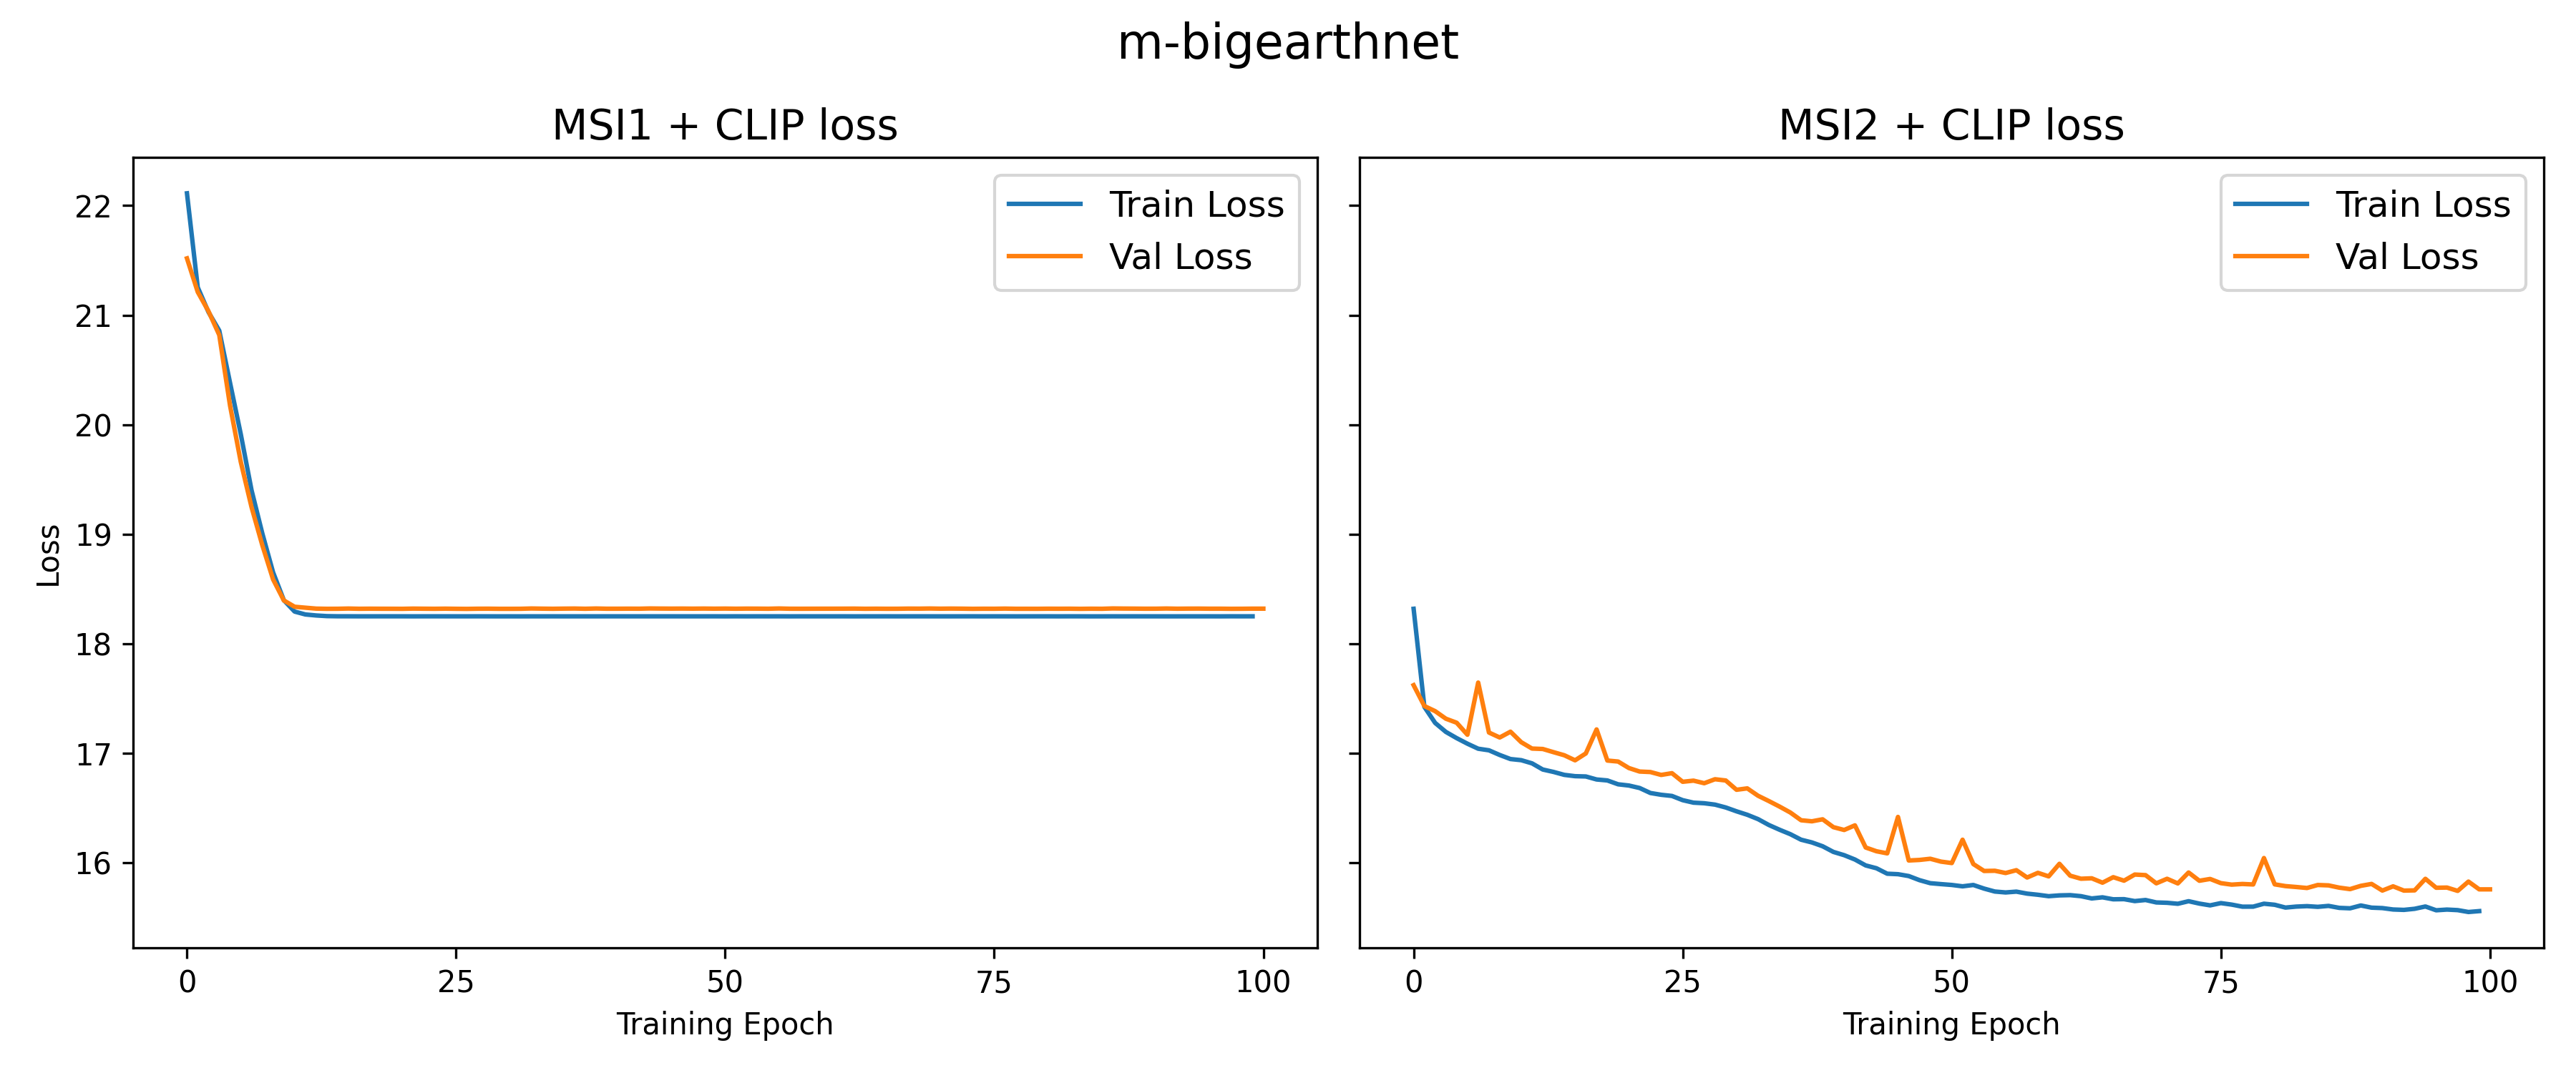
\includegraphics[width=\textwidth]{img/m-bigearthnet_loss_plot.png}
    \caption{Training and validation loss of the two embedders on the m-bigearthnet dataset from GEO-Bench.}
    \label{fig:benloss}
\end{figure}




\chapter{Conclusions} % ---------------------------------------

Recap key findings.

Acknowledge limitations: no full retraining of CLIP, only ViT-B/32, etc.

Propose future work: test on ViT-L/14, use other datasets (e.g., SEN12MS), explore better MSI fusion methods (e.g., attention mechanisms), or extend to segmentation.

Conclusions on the work results, discussion of potential future directions (applying the MSI Embedder to a RS-specialized CLIP, trying different models)

Future work directions: hyperparameter tuning, trying bigger embedders, multilabel classification model to be restructured according to what said in that paper (maybe trying something like that with GeoRSCLIP or so, ...

Also see last chapters of the Pi School report



\cleardoublepage

% APPENDIX ----------------------------------------------------
\appendix
\chapter{Additional results}


\begin{table}[ht]
\centering
\footnotesize
\renewcommand{\arraystretch}{1.2}
    \begin{tabular}{cccccc|c}
    \toprule
    %\textbf{Model} & \textbf{Method} & \multicolumn{5}{c}{\textbf{m-bigearthnet}} \\
    \multirow{2}{*}{\textbf{Model}} & \multirow{2}{*}{\textbf{Method}} & \multicolumn{5}{c}{\textbf{m-bigearthnet}} \\
    \cmidrule(lr){3-7}
    & & \textbf{R@5} & \textbf{P@5} & \textbf{mAP} & \textbf{F1} & \textbf{rloss} \\
    \specialrule{.06em}{.2em}{.2em}
    CLIP & zero-shot & \textbf{31.70\%} &  \textbf{23.40\%} & \textbf{32.32\%} & \textbf{20.39\%} & \textbf{28.71\%} \\
    | &  | & | & | & | &| & | \\
    MSI1 & finetune & 19.99\% & 15.58\% & 24.57\% & 15.29\% & 39.82\% \\
    MSI2 & finetune & 15.58\% & 11.46\% & 19.44\% & 14.55\% & 45.53\% \\
    MSI-T-s & zero shot & 15.95\% & 12.84\% & 20.36\% & 16.46\% & 42.26\% \\
    MSI-T-E & zero shot & \underline{29.56\%1} & \underline{22.24\%} & \underline{30.90\%} & \underline{20.30\%} & \underline{28.58\%} \\
    MSI-T-E-4L & zero shot & 24.61\% & 19.02\% & 27.51\% & 19.23\% & 33.45\% \\
    \bottomrule
    \end{tabular}
\vspace{0.3cm}
\caption{\normalsize Performance of models on the m-bigearthnet dataset across various evaluation metrics: the accuracy in bold refers to the best performing model, the underlined one to the second best.}
\label{tab:mbigearthnetresults}
\end{table}

\backmatter

% BIBLIOGRAPHY ------------------------------------------------
\newpage
\phantomsection % use this command only if hyperref is loaded
\addcontentsline{toc}{chapter}{\bibname}
% Here put the code for the bibliography. You can use BibTeX or
% the BibLaTeX package or the simple environment thebibliography.
\bibliographystyle{unsrt} % style can be changed
% 'unsrt' is identical to 'plain', but disables the automatic alphabetical order
\bibliography{references.bib}

\end{document}
